\documentclass[11pt,fleqn]{book} % Default font size and left-justified equations
%%%%%%%%%%%%%%%%%%%%%%%%%%%%%%%%%%%%%%%%%
% The Legrand Orange Book
% Structural Definitions File
% Version 2.0 (9/2/15)
%
% Original author:
% Mathias Legrand (legrand.mathias@gmail.com) with modifications by:
% Vel (vel@latextemplates.com)
% 
% This file has been downloaded from:
% http://www.LaTeXTemplates.com
%
% License:
% CC BY-NC-SA 3.0 (http://creativecommons.org/licenses/by-nc-sa/3.0/)
%
%%%%%%%%%%%%%%%%%%%%%%%%%%%%%%%%%%%%%%%%%

%----------------------------------------------------------------------------------------
%	VARIOUS REQUIRED PACKAGES AND CONFIGURATIONS
%----------------------------------------------------------------------------------------

\usepackage[top=3cm,bottom=3cm,left=3cm,right=3cm,headsep=10pt,a4paper]{geometry} % Page margins

\usepackage{graphicx} % Required for including pictures
\graphicspath{{Pictures/}} % Specifies the directory where pictures are stored

\usepackage{lipsum} % Inserts dummy text

\usepackage{tikz} % Required for drawing custom shapes

\usepackage[spanish,activeacute,es-tabla]{babel}
%\usepackage[english]{babel} % English language/hyphenation

\usepackage{enumitem} % Customize lists
\setlist{nolistsep} % Reduce spacing between bullet points and numbered lists

\usepackage{booktabs} % Required for nicer horizontal rules in tables

\usepackage{xcolor} % Required for specifying colors by name
\definecolor{ocre}{RGB}{243,102,25} % Define the orange color used for highlighting throughout the book

%----------------------------------------------------------------------------------------
%	FONTS
%----------------------------------------------------------------------------------------

\usepackage{avant} % Use the Avantgarde font for headings
%\usepackage{times} % Use the Times font for headings
\usepackage{mathptmx} % Use the Adobe Times Roman as the default text font together with math symbols from the Sym­bol, Chancery and Com­puter Modern fonts

\usepackage{microtype} % Slightly tweak font spacing for aesthetics
\usepackage[utf8]{inputenc} % Required for including letters with accents
\usepackage[T1]{fontenc} % Use 8-bit encoding that has 256 glyphs

%----------------------------------------------------------------------------------------
%	BIBLIOGRAPHY AND INDEX
%----------------------------------------------------------------------------------------

\usepackage[style=alphabetic,citestyle=numeric,sorting=nyt,sortcites=true,
            autopunct=true,babel=hyphen,hyperref=true,abbreviate=false,
            backref=true,backend=biber]{biblatex}
\addbibresource{bibliography} % BibTeX bibliography file
\defbibheading{bibempty}{}

\usepackage{calc} % For simpler calculation - used for spacing the index letter headings correctly
\usepackage{makeidx} % Required to make an index
\makeindex % Tells LaTeX to create the files required for indexing

%----------------------------------------------------------------------------------------
%	MAIN TABLE OF CONTENTS
%----------------------------------------------------------------------------------------

\usepackage{titletoc} % Required for manipulating the table of contents

\contentsmargin{0cm} % Removes the default margin

% Part text styling
\titlecontents{part}[0cm]
{\addvspace{20pt}\centering\large\bfseries}
{}
{}
{}

% Chapter text styling
\titlecontents{chapter}[1.25cm] % Indentation
{\addvspace{12pt}\large\sffamily\bfseries} % Spacing and font options for chapters
{\color{ocre!60}\contentslabel[\Large\thecontentslabel]{1.25cm}\color{ocre}} % Chapter number
{\color{ocre}}  
{\color{ocre!60}\normalsize\;\titlerule*[.5pc]{.}\;\thecontentspage} % Page number

% Section text styling
\titlecontents{section}[1.25cm] % Indentation
{\addvspace{3pt}\sffamily\bfseries} % Spacing and font options for sections
{\contentslabel[\thecontentslabel]{1.25cm}} % Section number
{}
{\hfill\color{black}\thecontentspage} % Page number
[]

% Subsection text styling
\titlecontents{subsection}[1.25cm] % Indentation
{\addvspace{1pt}\sffamily\small} % Spacing and font options for subsections
{\contentslabel[\thecontentslabel]{1.25cm}} % Subsection number
{}
{\ \titlerule*[.5pc]{.}\;\thecontentspage} % Page number
[]

% List of figures
\titlecontents{figure}[0em]
{\addvspace{-5pt}\sffamily}
{\thecontentslabel\hspace*{1em}}
{}
{\ \titlerule*[.5pc]{.}\;\thecontentspage}
[]

% List of tables
\titlecontents{table}[0em]
{\addvspace{-5pt}\sffamily}
{\thecontentslabel\hspace*{1em}}
{}
{\ \titlerule*[.5pc]{.}\;\thecontentspage}
[]

%----------------------------------------------------------------------------------------
%	MINI TABLE OF CONTENTS IN PART HEADS
%----------------------------------------------------------------------------------------

% Chapter text styling
\titlecontents{lchapter}[0em] % Indenting
{\addvspace{15pt}\large\sffamily\bfseries} % Spacing and font options for chapters
{\color{ocre}\contentslabel[\Large\thecontentslabel]{1.25cm}\color{ocre}} % Chapter number
{}  
{\color{ocre}\normalsize\sffamily\bfseries\;\titlerule*[.5pc]{.}\;\thecontentspage} % Page number

% Section text styling
\titlecontents{lsection}[0em] % Indenting
{\sffamily\small} % Spacing and font options for sections
{\contentslabel[\thecontentslabel]{1.25cm}} % Section number
{}
{}

% Subsection text styling
\titlecontents{lsubsection}[.5em] % Indentation
{\normalfont\footnotesize\sffamily} % Font settings
{}
{}
{}

%----------------------------------------------------------------------------------------
%	PAGE HEADERS
%----------------------------------------------------------------------------------------

\usepackage{fancyhdr} % Required for header and footer configuration

\pagestyle{fancy}
\renewcommand{\chaptermark}[1]{\markboth{\sffamily\normalsize\bfseries\chaptername\ \thechapter.\ #1}{}} % Chapter text font settings
\renewcommand{\sectionmark}[1]{\markright{\sffamily\normalsize\thesection\hspace{5pt}#1}{}} % Section text font settings
\fancyhf{} \fancyhead[LE,RO]{\sffamily\normalsize\thepage} % Font setting for the page number in the header
\fancyhead[LO]{\rightmark} % Print the nearest section name on the left side of odd pages
\fancyhead[RE]{\leftmark} % Print the current chapter name on the right side of even pages
\renewcommand{\headrulewidth}{0.5pt} % Width of the rule under the header
\addtolength{\headheight}{2.5pt} % Increase the spacing around the header slightly
\renewcommand{\footrulewidth}{0pt} % Removes the rule in the footer
\fancypagestyle{plain}{\fancyhead{}\renewcommand{\headrulewidth}{0pt}} % Style for when a plain pagestyle is specified

% Removes the header from odd empty pages at the end of chapters
\makeatletter
\renewcommand{\cleardoublepage}{
\clearpage\ifodd\c@page\else
\hbox{}
\vspace*{\fill}
\thispagestyle{empty}
\newpage
\fi}

%----------------------------------------------------------------------------------------
%	THEOREM STYLES
%----------------------------------------------------------------------------------------

\usepackage{amsmath,amsfonts,amssymb,amsthm} % For math equations, theorems, symbols, etc

\newcommand{\intoo}[2]{\mathopen{]}#1\,;#2\mathclose{[}}
\newcommand{\ud}{\mathop{\mathrm{{}d}}\mathopen{}}
\newcommand{\intff}[2]{\mathopen{[}#1\,;#2\mathclose{]}}
\newtheorem{notation}{Notation}[chapter]

% Boxed/framed environments
\newtheoremstyle{ocrenumbox}% % Theorem style name
{0pt}% Space above
{0pt}% Space below
{\normalfont}% % Body font
{}% Indent amount
{\small\bf\sffamily\color{ocre}}% % Theorem head font
{\;}% Punctuation after theorem head
{0.25em}% Space after theorem head
{\small\sffamily\color{ocre}\thmname{#1}\nobreakspace\thmnumber{\@ifnotempty{#1}{}\@upn{#2}}% Theorem text (e.g. Theorem 2.1)
\thmnote{\nobreakspace\the\thm@notefont\sffamily\bfseries\color{black}---\nobreakspace#3.}} % Optional theorem note
\renewcommand{\qedsymbol}{$\blacksquare$}% Optional qed square

\newtheoremstyle{blacknumex}% Theorem style name
{5pt}% Space above
{5pt}% Space below
{\normalfont}% Body font
{} % Indent amount
{\small\bf\sffamily}% Theorem head font
{\;}% Punctuation after theorem head
{0.25em}% Space after theorem head
{\small\sffamily{\tiny\ensuremath{\blacksquare}}\nobreakspace\thmname{#1}\nobreakspace\thmnumber{\@ifnotempty{#1}{}\@upn{#2}}% Theorem text (e.g. Theorem 2.1)
\thmnote{\nobreakspace\the\thm@notefont\sffamily\bfseries---\nobreakspace#3.}}% Optional theorem note

\newtheoremstyle{blacknumbox} % Theorem style name
{0pt}% Space above
{0pt}% Space below
{\normalfont}% Body font
{}% Indent amount
{\small\bf\sffamily}% Theorem head font
{\;}% Punctuation after theorem head
{0.25em}% Space after theorem head
{\small\sffamily\thmname{#1}\nobreakspace\thmnumber{\@ifnotempty{#1}{}\@upn{#2}}% Theorem text (e.g. Theorem 2.1)
\thmnote{\nobreakspace\the\thm@notefont\sffamily\bfseries---\nobreakspace#3.}}% Optional theorem note

% Non-boxed/non-framed environments
\newtheoremstyle{ocrenum}% % Theorem style name
{5pt}% Space above
{5pt}% Space below
{\normalfont}% % Body font
{}% Indent amount
{\small\bf\sffamily\color{ocre}}% % Theorem head font
{\;}% Punctuation after theorem head
{0.25em}% Space after theorem head
{\small\sffamily\color{ocre}\thmname{#1}\nobreakspace\thmnumber{\@ifnotempty{#1}{}\@upn{#2}}% Theorem text (e.g. Theorem 2.1)
\thmnote{\nobreakspace\the\thm@notefont\sffamily\bfseries\color{black}---\nobreakspace#3.}} % Optional theorem note
\renewcommand{\qedsymbol}{$\blacksquare$}% Optional qed square
\makeatother

% Defines the theorem text style for each type of theorem to one of the three styles above
\newcounter{dummy} 
\numberwithin{dummy}{section}
\theoremstyle{ocrenumbox}
\newtheorem{theoremeT}[dummy]{Theorem}
\newtheorem{problem}{Problema}[chapter]    %CAMBIADO
\newtheorem{exerciseT}{Ejercicio}[chapter] %CAMBIADO
\theoremstyle{blacknumex}
\newtheorem{exampleT}{Ejemplo}[chapter]   %CAMBIADO
\theoremstyle{blacknumbox}
\newtheorem{vocabulary}{Vocabulary}[chapter]
\newtheorem{definitionT}{Definición}[section] %CAMBIADO
\newtheorem{corollaryT}[dummy]{Corollary}
\theoremstyle{ocrenum}
\newtheorem{proposition}[dummy]{Proposition}

%----------------------------------------------------------------------------------------
%	DEFINITION OF COLORED BOXES
%----------------------------------------------------------------------------------------

\RequirePackage[framemethod=default]{mdframed} % Required for creating the theorem, definition, exercise and corollary boxes

% Theorem box
\newmdenv[skipabove=7pt,
skipbelow=7pt,
backgroundcolor=black!5,
linecolor=ocre,
innerleftmargin=5pt,
innerrightmargin=5pt,
innertopmargin=5pt,
leftmargin=0cm,
rightmargin=0cm,
innerbottommargin=5pt]{tBox}

% Exercise box	  
\newmdenv[skipabove=7pt,
skipbelow=7pt,
rightline=false,
leftline=true,
topline=false,
bottomline=false,
backgroundcolor=ocre!10,
linecolor=ocre,
innerleftmargin=5pt,
innerrightmargin=5pt,
innertopmargin=5pt,
innerbottommargin=5pt,
leftmargin=0cm,
rightmargin=0cm,
linewidth=4pt]{eBox}	

% Definition box
\newmdenv[skipabove=7pt,
skipbelow=7pt,
rightline=false,
leftline=true,
topline=false,
bottomline=false,
linecolor=ocre,
innerleftmargin=5pt,
innerrightmargin=5pt,
innertopmargin=0pt,
leftmargin=0cm,
rightmargin=0cm,
linewidth=4pt,
innerbottommargin=0pt]{dBox}	

% Corollary box
\newmdenv[skipabove=7pt,
skipbelow=7pt,
rightline=false,
leftline=true,
topline=false,
bottomline=false,
linecolor=gray,
backgroundcolor=black!5,
innerleftmargin=5pt,
innerrightmargin=5pt,
innertopmargin=5pt,
leftmargin=0cm,
rightmargin=0cm,
linewidth=4pt,
innerbottommargin=5pt]{cBox}

% Creates an environment for each type of theorem and assigns it a theorem text style from the "Theorem Styles" section above and a colored box from above
\newenvironment{theorem}{\begin{tBox}\begin{theoremeT}}{\end{theoremeT}\end{tBox}}
\newenvironment{exercise}{\begin{eBox}\begin{exerciseT}}{\hfill{\color{ocre}\tiny\ensuremath{\blacksquare}}\end{exerciseT}\end{eBox}}				  
\newenvironment{definition}{\begin{dBox}\begin{definitionT}}{\end{definitionT}\end{dBox}}	
\newenvironment{example}{\begin{exampleT}}{\hfill{\tiny\ensuremath{\blacksquare}}\end{exampleT}}		
\newenvironment{corollary}{\begin{cBox}\begin{corollaryT}}{\end{corollaryT}\end{cBox}}	

%----------------------------------------------------------------------------------------
%	REMARK ENVIRONMENT
%----------------------------------------------------------------------------------------

\newenvironment{remark}{\par\vspace{10pt}\small % Vertical white space above the remark and smaller font size
\begin{list}{}{
\leftmargin=35pt % Indentation on the left
\rightmargin=25pt}\item\ignorespaces % Indentation on the right
\makebox[-2.5pt]{\begin{tikzpicture}[overlay]
\node[draw=ocre!60,line width=1pt,circle,fill=ocre!25,font=\sffamily\bfseries,inner sep=2pt,outer sep=0pt] at (-15pt,0pt){\textcolor{ocre}{R}};\end{tikzpicture}} % Orange R in a circle
\advance\baselineskip -1pt}{\end{list}\vskip5pt} % Tighter line spacing and white space after remark

%----------------------------------------------------------------------------------------
%	SECTION NUMBERING IN THE MARGIN
%----------------------------------------------------------------------------------------

\makeatletter
\renewcommand{\@seccntformat}[1]{\llap{\textcolor{ocre}{\csname the#1\endcsname}\hspace{1em}}}                    
\renewcommand{\section}{\@startsection{section}{1}{\z@}
{-4ex \@plus -1ex \@minus -.4ex}
{1ex \@plus.2ex }
{\normalfont\large\sffamily\bfseries}}
\renewcommand{\subsection}{\@startsection {subsection}{2}{\z@}
{-3ex \@plus -0.1ex \@minus -.4ex}
{0.5ex \@plus.2ex }
{\normalfont\sffamily\bfseries}}
\renewcommand{\subsubsection}{\@startsection {subsubsection}{3}{\z@}
{-2ex \@plus -0.1ex \@minus -.2ex}
{.2ex \@plus.2ex }
{\normalfont\small\sffamily\bfseries}}                        
\renewcommand\paragraph{\@startsection{paragraph}{4}{\z@}
{-2ex \@plus-.2ex \@minus .2ex}
{.1ex}
{\normalfont\small\sffamily\bfseries}}

%----------------------------------------------------------------------------------------
%	PART HEADINGS
%----------------------------------------------------------------------------------------

% numbered part in the table of contents
\newcommand{\@mypartnumtocformat}[2]{%
\setlength\fboxsep{0pt}%
\noindent\colorbox{ocre!20}{\strut\parbox[c][.7cm]{\ecart}{\color{ocre!70}\Large\sffamily\bfseries\centering#1}}\hskip\esp\colorbox{ocre!40}{\strut\parbox[c][.7cm]{\linewidth-\ecart-\esp}{\Large\sffamily\centering#2}}}%
%%%%%%%%%%%%%%%%%%%%%%%%%%%%%%%%%%
% unnumbered part in the table of contents
\newcommand{\@myparttocformat}[1]{%
\setlength\fboxsep{0pt}%
\noindent\colorbox{ocre!40}{\strut\parbox[c][.7cm]{\linewidth}{\Large\sffamily\centering#1}}}%
%%%%%%%%%%%%%%%%%%%%%%%%%%%%%%%%%%
\newlength\esp
\setlength\esp{4pt}
\newlength\ecart
\setlength\ecart{1.2cm-\esp}
\newcommand{\thepartimage}{}%
\newcommand{\partimage}[1]{\renewcommand{\thepartimage}{#1}}%
\def\@part[#1]#2{%
\ifnum \c@secnumdepth >-2\relax%
\refstepcounter{part}%
\addcontentsline{toc}{part}{\texorpdfstring{\protect\@mypartnumtocformat{\thepart}{#1}}{\partname~\thepart\ ---\ #1}}
\else%
\addcontentsline{toc}{part}{\texorpdfstring{\protect\@myparttocformat{#1}}{#1}}%
\fi%
\startcontents%
\markboth{}{}%
{\thispagestyle{empty}%
\begin{tikzpicture}[remember picture,overlay]%
\node at (current page.north west){\begin{tikzpicture}[remember picture,overlay]%	
\fill[ocre!20](0cm,0cm) rectangle (\paperwidth,-\paperheight);
\node[anchor=north] at (4cm,-3.25cm){\color{ocre!40}\fontsize{220}{100}\sffamily\bfseries\thepart}; 
\node[anchor=south east] at (\paperwidth-1cm,-\paperheight+1cm){\parbox[t][][t]{8.5cm}{
\printcontents{l}{0}{\setcounter{tocdepth}{0}} 
% CAMBIADO para que en la portada de cada capitulo solo salga la sección
}};
\node[anchor=north east] at (\paperwidth-1.5cm,-3.25cm){\parbox[t][][t]{15cm}{\strut\raggedleft\color{white}\fontsize{30}{30}\sffamily\bfseries#2}};
\end{tikzpicture}};
\end{tikzpicture}}%
\@endpart}
\def\@spart#1{%
\startcontents%
\phantomsection
{\thispagestyle{empty}%
\begin{tikzpicture}[remember picture,overlay]%
\node at (current page.north west){\begin{tikzpicture}[remember picture,overlay]%	
\fill[ocre!20](0cm,0cm) rectangle (\paperwidth,-\paperheight);
\node[anchor=north east] at (\paperwidth-1.5cm,-3.25cm){\parbox[t][][t]{15cm}{\strut\raggedleft\color{white}\fontsize{30}{30}\sffamily\bfseries#1}};
\end{tikzpicture}};
\end{tikzpicture}}
\addcontentsline{toc}{part}{\texorpdfstring{%
\setlength\fboxsep{0pt}%
\noindent\protect\colorbox{ocre!40}{\strut\protect\parbox[c][.7cm]{\linewidth}{\Large\sffamily\protect\centering #1\quad\mbox{}}}}{#1}}%
\@endpart}
\def\@endpart{\vfil\newpage
\if@twoside
\if@openright
\null
\thispagestyle{empty}%
\newpage
\fi
\fi
\if@tempswa
\twocolumn
\fi}

%----------------------------------------------------------------------------------------
%	CHAPTER HEADINGS
%----------------------------------------------------------------------------------------

% A switch to conditionally include a picture, implemented by  Christian Hupfer
\newif\ifusechapterimage
\usechapterimagetrue
\newcommand{\thechapterimage}{}%
\newcommand{\chapterimage}[1]{\ifusechapterimage\renewcommand{\thechapterimage}{#1}\fi}%
\newcommand{\autodot}{.}
\def\@makechapterhead#1{%
{\parindent \z@ \raggedright \normalfont
\ifnum \c@secnumdepth >\m@ne
\if@mainmatter
\begin{tikzpicture}[remember picture,overlay]
\node at (current page.north west)
{\begin{tikzpicture}[remember picture,overlay]
\node[anchor=north west,inner sep=0pt] at (0,0) {\ifusechapterimage\includegraphics[width=\paperwidth]{\thechapterimage}\fi};
\draw[anchor=west] (\Gm@lmargin,-9cm) node [line width=2pt,rounded corners=15pt,draw=ocre,fill=white,fill opacity=0.5,inner sep=15pt]{\strut\makebox[22cm]{}};
\draw[anchor=west] (\Gm@lmargin+.3cm,-9cm) node {\huge\sffamily\bfseries\color{black}\thechapter\autodot~#1\strut};
\end{tikzpicture}};
\end{tikzpicture}
\else
\begin{tikzpicture}[remember picture,overlay]
\node at (current page.north west)
{\begin{tikzpicture}[remember picture,overlay]
\node[anchor=north west,inner sep=0pt] at (0,0) {\ifusechapterimage\includegraphics[width=\paperwidth]{\thechapterimage}\fi};
\draw[anchor=west] (\Gm@lmargin,-9cm) node [line width=2pt,rounded corners=15pt,draw=ocre,fill=white,fill opacity=0.5,inner sep=15pt]{\strut\makebox[22cm]{}};
\draw[anchor=west] (\Gm@lmargin+.3cm,-9cm) node {\huge\sffamily\bfseries\color{black}#1\strut};
\end{tikzpicture}};
\end{tikzpicture}
\fi\fi\par\vspace*{270\p@}}}

%-------------------------------------------

\def\@makeschapterhead#1{%
\begin{tikzpicture}[remember picture,overlay]
\node at (current page.north west)
{\begin{tikzpicture}[remember picture,overlay]
\node[anchor=north west,inner sep=0pt] at (0,0) {\ifusechapterimage\includegraphics[width=\paperwidth]{\thechapterimage}\fi};
\draw[anchor=west] (\Gm@lmargin,-9cm) node [line width=2pt,rounded corners=15pt,draw=ocre,fill=white,fill opacity=0.5,inner sep=15pt]{\strut\makebox[22cm]{}};
\draw[anchor=west] (\Gm@lmargin+.3cm,-9cm) node {\huge\sffamily\bfseries\color{black}#1\strut};
\end{tikzpicture}};
\end{tikzpicture}
\par\vspace*{270\p@}}
\makeatother

%----------------------------------------------------------------------------------------
%	HYPERLINKS IN THE DOCUMENTS
%----------------------------------------------------------------------------------------

\usepackage{hyperref}
\hypersetup{hidelinks,backref=true,pagebackref=true,hyperindex=true,colorlinks=false,breaklinks=true,urlcolor= ocre,bookmarks=true,bookmarksopen=false,pdftitle={Title},pdfauthor={Author}}
\usepackage{bookmark}
\bookmarksetup{
open,
numbered,
addtohook={%
\ifnum\bookmarkget{level}=0 % chapter
\bookmarksetup{bold}%
\fi
\ifnum\bookmarkget{level}=-1 % part
\bookmarksetup{color=ocre,bold}%
\fi
}
}

%----------------------------------------------------------------------------------------
%	LISTADOS
%----------------------------------------------------------------------------------------
\usepackage{color}
\definecolor{gray97}{gray}{.97}
\definecolor{gray75}{gray}{.75}
\definecolor{gray45}{gray}{.45}

\usepackage{listings}
\lstset{
language=C,
frame=Ltb,
framerule=0pt,
aboveskip=0.5cm,
framextopmargin=3pt,
framexbottommargin=3pt,
framexleftmargin=0.4cm,
framesep=0pt,
rulesep=.4pt,
backgroundcolor=\color{gray97},
rulesepcolor=\color{black},
tabsize=2,
numbers=left,
numbersep=15pt,
numberstyle=\tiny,
numberfirstline = false,
breaklines=true,
%
identifierstyle=\color{blue},
stringstyle=\color{orange},
basicstyle=\footnotesize\ttfamily,
keywordstyle=\bfseries\color{green!40!black},
commentstyle=\itshape\color{purple!40!black},
%
showstringspaces = false,
commentstyle=\color{gray45},
literate=%
         {á}{{\'a}}1
         {é}{{\'a}}1
         {í}{{\'i}}1
         {ó}{{\'o}}1
         {ú}{{\'u}}1
         {ñ}{{\~n}}1
}

%----------------------------------------------------------------------------------------
%	MIS COSAS
%----------------------------------------------------------------------------------------
%\setlength{\parskip}{\baselineskip} % espaciado entre parrafos
\usepackage{subfig}

\begin{document}

%----------------------------------------------------------------------------------
% TITLE PAGE
%----------------------------------------------------------------------------------
\begingroup
\thispagestyle{empty}
\begin{tikzpicture}[remember picture,overlay]
\node[inner sep=0pt] (background) at (current page.center) {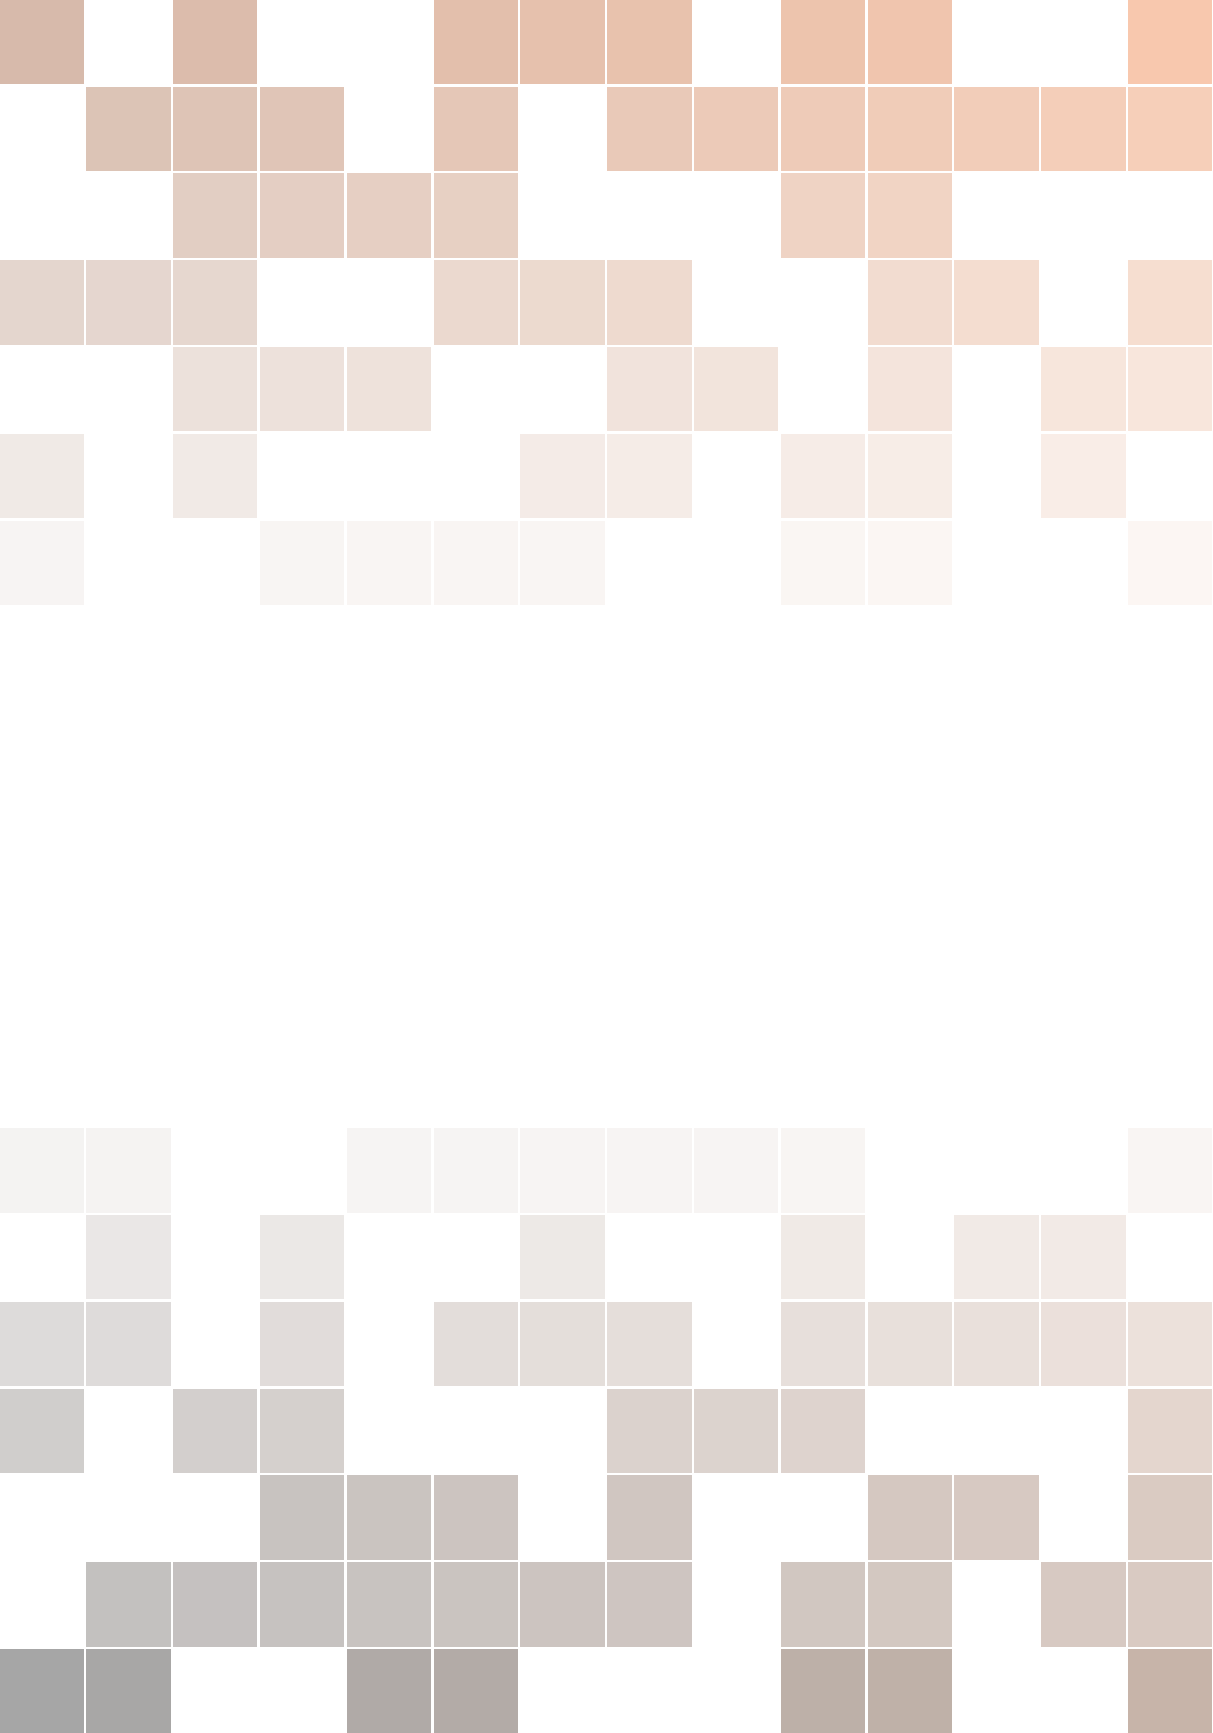
\includegraphics[width=\paperwidth]{background}};
\draw (current page.center) node [fill=ocre!30!white,fill opacity=0.6,text opacity=1,inner sep=1cm]
{\Huge\centering\bfseries\sffamily\parbox[c][][t]{\paperwidth}{\centering Programación de la Consola Nintendo DS\\[15pt] % Book title
{\Large VJ1214 Consolas y dispositivos de videojuegos \\ Grado en Diseño y Desarrollo de Videojuegos}\\[20pt] % Subtitle
{\huge Raúl Montoliu Colas\\ Juan Carlos Fernández Fernández\\ Maribel Castillo Catalán}}}; % Author name
\end{tikzpicture}
\vfill
\endgroup

%---------------------------------------------------------------------------------
% COPYRIGHT PAGE
%----------------------------------------------------------------------------------
\newpage
~\vfill
\thispagestyle{empty}

\noindent Copyright \copyright 2018 Raúl Montoliu Colas, Juan Carlos Fernández Fernández, Maribel Castillo Catalán. \\
\noindent Esta obra se distribuye bajo la Licencia \textit{Creative Commons Atribución-Compartir Igual 4.0 Internacional}. Puede consultar las condiciones de dicha licencia en: \url{http://creativecommons.org/licenses/by-sa/4.0/} \\

\includegraphics{Figuras/by-sa.png} 

%----------------------------------------------------------------------------------
% TABLE OF CONTENTS
%----------------------------------------------------------------------------------
\usechapterimagefalse % If you don't want to include a chapter image, use this to toggle images off - it can be enabled later with \usechapterimagetrue

\chapterimage{chapter_head_1.pdf} % Table of contents heading image
\pagestyle{empty} % No headers
\setcounter{tocdepth}{1} %Capitulos y secciones
\tableofcontents % Print the table of contents itself
\cleardoublepage % Forces the first chapter to start on an odd page so it's on the right
\pagestyle{fancy} % Print headers again

%----------------------------------------------------------------------------------
% CHAPTERS
%----------------------------------------------------------------------------------
\chapterimage{chapter_head_1.pdf} 
\chapter{Introducción a la consola Nintendo DS}

Este capítulo expone, en primer lugar, el conjunto de consolas de la familia Nintendo y posteriormente describe los principales elementos Hardware de la computadora Nintendo DS, que es la videoconsola a la que se hace referencia en el resto de los capítulos de este libro.

% -----------------------------------------------------------------
% -----------------------------------------------------------------
% -----------------------------------------------------------------
% -----------------------------------------------------------------
\section{Las videoconsolas de Nintendo}

Existe una amplia variedad de consolas de Nintendo:

\begin{itemize}
\item \textit{GameBoy Advance (GBA)}: tiene un procesador \textit{ARM7TDMI}, de 32 	bits, junto con un procesador \textit{Z80}, para dar soporte a los juegos de la \textit{GameBoy} clásica (ver Figura \ref{fig_c1_nintendo1}a). 
%
\item \textit{Nintendo DS (NDS)}: tiene un procesador ARM9 a 66Mhz y un procesador ARM7 a 33Mhz (ver Figura \ref{fig_c1_nintendo1}b).
%	
\item \textit{Nintendo DS Lite}: se diferencia de la NDS normal en su aspecto más estilizado, en mejoras de consumo energético y los diferentes niveles de control de brillo de la pantalla (ver Figura \ref{fig_c1_nintendo2}a). 
%	
\item \textit{Nintendo DSi}: incorpora dos cámaras de baja resolución, pantallas ligeramente mayores, mejor sonido, más memoria y una nueva ranura para tarjetas \textit{Secure Digital (SD)}. A cambio pierde la ranura de compa\-ti\-bilidad con los cartuchos de \textit{GameBoy	Advance (Slot2)} (ver Figura \ref{fig_c1_nintendo2}b).
%
\item \textit{Nintendo DSi XL}: conocida también como \textit{DSi XL}, es prácticamente idéntica a la anterior, salvo que su forma es significativamente mayor. 
%
\item \textit{Nintendo 3DS}: permite jugar con juegos y ver películas en 3D. Además, la nueva pantalla ofrece imágenes estereoscópicas sin necesidad de gafas especiales para disfrutar del efecto 3D. Incorpora una pantalla táctil, red inalámbrica ()\textit{WiFi}), sensor de movimiento con giroscopio de tres ejes y acelerómetro de tres ejes (ver Figura \ref{fig_c1_nintendo3}a).
%
\item \textit{Nintendo 2DS}: conserva las mismas funciones y especificaciones que la \textit{Nintendo 3DS}, salvo que no reproduce los videojuegos con efecto 3D, sino en 2D. Además, mantiene el tamaño de las pantallas de la \textit{Nintendo 3DS} (ver Figura \ref{fig_c1_nintendo3}b).
%	
\item \textit{New Nintendo 3DS}: esta consola cuenta con botones de colores.  Las pantallas de la \textit{New Nintendo 3DS} son 1,2 veces más grandes que las de la \textit{Nintendo 3DS} original, mientras que el tamaño de las pantallas de la \textit{New Nintendo 3DS XL} son similares a las de su predecesora. (ver Figura \ref{fig_c1_nintendo3}c). Las ranuras de la tarjeta de juego, del lápiz y del botón de encendido se han trasladado a la base de la consola. Como nuevas características cabe destacar:
	\begin{itemize}
		\item El rastreo facial para que la cámara siga la línea de visión del jugador, de esta forma se amplía la gama de ángulos desde los que se puede ver el efecto 3D estereoscópico del sistema.
		\item La variación automática del brillo de las pantallas según la iluminación ambiental.
		\item La transferencia inalámbrica de archivos multimedia entre la consola y un ordenador.
		\item Una CPU más potente, un ARM11 Dual Core a 532MHz. 
	\end{itemize}	
\end{itemize}


\begin{figure}
	\centering
	\subfloat[\textit{GameBoy Advance}]{
		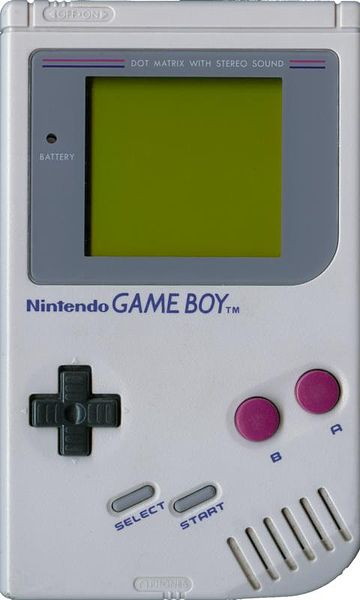
\includegraphics[height=5cm]{./Figuras/C1/c1_360px-Gameboy.jpg}}
	\subfloat[\textit{Nintendo DS}]{
		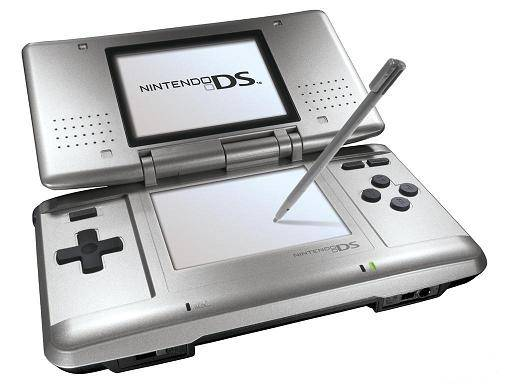
\includegraphics[height=5cm]{./Figuras/C1/c1_Nintendo_ds.jpg}}
	\caption{Videoconsolas de Nintendo: GBA y NDS}
	\label{fig_c1_nintendo1}
\end{figure}

\begin{figure}
	\centering
	\subfloat[\textit{Nintendo DS Lite}]{
		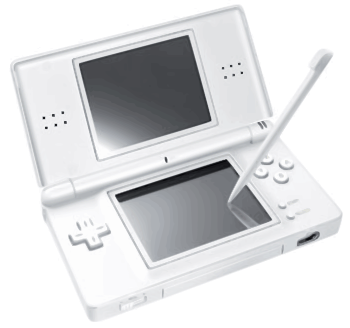
\includegraphics[height=5cm]{./Figuras/C1/c1_Nintendo-ds-lite.png}}
	\subfloat[\textit{Nintendo DSi}]{
		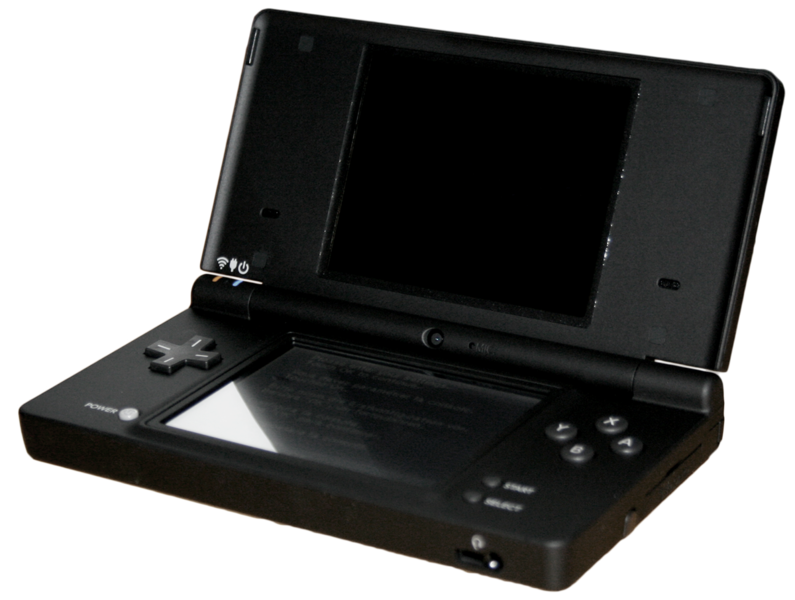
\includegraphics[height=5cm]{./Figuras/C1/c1_Nintendo_DSi.png}}
	\caption{Videoconsolas de Nintendo: NDSLite y NDSi}
	\label{fig_c1_nintendo2}
\end{figure}

\begin{figure}
	\centering
	\subfloat[\textit{Nintendo 3DS}]{
		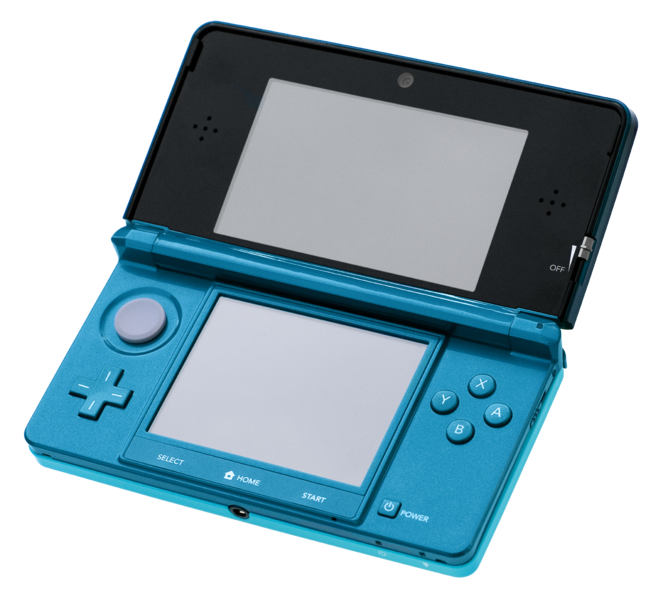
\includegraphics[height=4cm]{./Figuras/C1/c1_663px-Nintendo-3DS-AquaOpen.png}}
	\subfloat[\textit{Nintendo 2DS}]{
		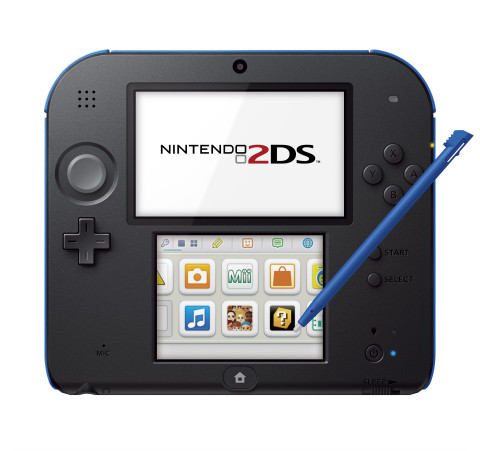
\includegraphics[height=4cm]{./Figuras/C1/c1_nintendo-2ds.jpg}}
	\subfloat[\textit{New Nintendo 3DS}]{
		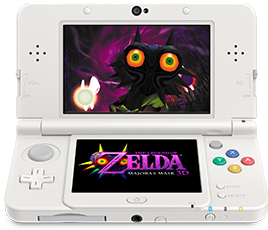
\includegraphics[height=4cm]{./Figuras/C1/c1_new-nintendo.png}}	
	\caption{Videoconsolas de Nintendo: N3DS, N2DS y NNew3DS}
	\label{fig_c1_nintendo3}
\end{figure}

% -----------------------------------------------------------------
% -----------------------------------------------------------------
% -----------------------------------------------------------------
% -----------------------------------------------------------------
\section{Hardware de la Nintendo DS (NDS)}

A continuación se describe el hardware de la \textit{Nintendo DS}:

\begin{itemize}
\item \textbf{Procesadores}: cuenta con dos procesadores, un ARM9 y un ARM7. El procesador ARM9 se encarga de la	lógica principal del programa, mientras que el ARM7, como procesador secundario, se encarga básicamente de gestionar el audio, la red inalámbrica (\textit{WiFi}) y algunas teclas. El hecho de que la consola NDS cuente con dos procesadores implica	la generación de dos ejecutables distintos, uno para cada procesador. El ejecutable del ARM7 actúa como esclavo del ARM9, atendiendo peticiones de reproducción de sonido o comunicaciones vía WiFi.
%	
\item \textbf{Memorias}:
	\begin{itemize}
	\item Memoria principal: tiene un tamaño de 4 MB. Dicha	memoria almacena el ejecutable para el ARM9, así como la gran mayoría de datos del ejecutable. Ambos procesadores pueden acceder a esta memoria en cualquier momento. Si ambos intentan acceder a la vez, será el que tenga mayor prioridad el que accede, quedando el otro a la espera.
	%
	\item Memoria de vídeo \textit{VRAM}: tiene  656 KB  distribuidos en  9 bancos de memoria de vídeo, que se pueden usar con diferentes propósitos. A lo largo de las sesiones de prácticas se verán más detalles de esta memoria de vídeo.
	%
	\item Otras memorias: tiene las pseudo-cachés \textit{WRAM} e \textit{IWRAM} de 96Kb, una memoria \textit{RAM} adicional para la \textit{BIOS} y una memoria virtual para vídeo (\textit{Virtual Video RAM}). 
	\end{itemize}
%
\item \textbf{Gráficos}: el hardware de vídeo se compone de dos núcleos gráficos 2D, uno	principal (\textit{main}) y otro secundario (\textit{sub}). Dichos núcleos se diferencian únicamente en que el motor principal puede \textit{renderizar} tanto la memoria de vídeo virtual sin utilizar el motor 2D, como mapas de bits de 256 colores, así como utilizar el motor 3D para el renderizado de alguno de sus fondos.
%
\item \textbf{Sonido}: dispone de altavoces estéreo y cuenta con 16 canales de audio independientes.
%
\item \textbf{Comunicación inalámbrica}: soporta el estándar de protocolo de comunicaciones \textit{IEEE 802.11}. El rango de comunicación inalámbrica varía de 10 a 30 metros, dependiendo de las circunstancias.
%
\item \textbf{Entrada/Salida}: tiene un puerto para cartuchos de juegos de Nintendo DS y otro para juegos de Game Boy Advance2. La NDS cuenta con una entrada para auriculares estéreo y otra entrada para micrófono.
%
\item \textbf{Doble pantalla}: las dos pantallas LCD son de 3 pulgadas. La pantalla inferior emplea tecnología táctil.
%
\item \textbf{Temporizador}: cuenta con un reloj de tiempo de real, que puede ser utilizado por una aplicación o juego para definir diferentes respuestas dependiendo de la hora del día.
\end{itemize}
 % Introducción a la consola Nintendo DS
\chapterimage{chapter_head_1.pdf} 
\chapter{Herramientas para programar la NDS}

Este capítulo está dedicado a la instalación de las herramientas necesarias para poder realizar videojuegos en la consola Nintendo DS. Así mismo se verá como poder realizar un primer programa \textit{Hello World}.

% --------------------------------------------------------------------------
% --------------------------------------------------------------------------
% --------------------------------------------------------------------------
% --------------------------------------------------------------------------
\section{Herramientas de desarrollo para programar con la NDS}

% --------------------------------------------------------------------------
% --------------------------------------------------------------------------
\subsection{Introducción}
Se denomina \textit{homebrew} al software \textit{casero} no oficial realizado por programadores, ya sean aficionados o expertos, para cualquier plataforma. Generalmente, esta plataforma suele ser una videoconsola pro\-pie\-taria. El desarrollo de software \textit{casero} está permitido en cualquiera de las consolas de Nintendo, siempre y cuando sea sin ánimo de lucro. En cualquier caso, se debe señalar que no todas las plataformas permiten el \textit{homebrew}. El desarrollo de software para la Nintendo DS se puede realizar de dos maneras diferentes:

\begin{itemize}
\item Utilizando el kit comercial de desarrollo de software (\textit{SDK}) de Nintendo.
\item Utilizando \textit{DevkitPro}, que es un conjunto de bibliotecas, compiladores y utilidades para desarrollar software para varias plataformas. Además, es libre y de descarga gratuita.
\end{itemize}

En los apartados siguientes de esta sección se presentarán las principales herramientas existentes que ayudan al desarrollo de aplicaciones para NDS.

% --------------------------------------------------------------------------
% --------------------------------------------------------------------------
\subsection{DevkitPro}
\textit{DevkitPro} es un conjunto de bibliotecas, compiladores y utilidades que permiten
desarrollar aplicaciones para las consolas \textit{Game Boy Advance (GBA)}, \textit{GP32}, \textit{GP2X}, \textit{Playstation Portable (PSP)}, \textit{Nintendo DS} y \textit{GameCube}. \textit{DekvitPro} cuenta con cuatro \textit{toolchains} que permiten escribir aplicaciones y juegos para las consolas citadas:

\begin{itemize}
\item \textit{DevkitARM}: utilizado para el desarrollo de aplicaciones para \textit{GBA},
\textit{GP32} y \textit{Nintendo DS}.
%
\item \textit{DevkitGP2X}: utilizado para el desarrollo de aplicaciones para la \textit{GamePark
GP2X}.
%
\item \textit{DevkitPPC}: utilizado para el desarrollo de aplicaciones para la \textit{Nintendo
GameCube}.
\item \textit{DevkitPSP}: utilizado para el desarrollo de aplicaciones para la \textit{Sony
PSP}.
\end{itemize}

% --------------------------------------------------------------------------
% --------------------------------------------------------------------------
\subsection{DevkitARM}
\textit{DevkitARM} es un \textit{toolchain} de los lenguajes \textit{C} y \textit{C++}, basado en la colección de compiladores \textit{GNU (GCC)}, que permite crear binarios para la \textit{arquitectura ARM}. Incluye todo lo necesario para crear software para la \textit{Nintendo DS}, \textit{GBA} y \textit{GP32}. Las bibliotecas que incluye \textit{DevkitARM} son las siguientes:

\begin{itemize}
\item \textit{LibNDS}: anteriormente conocida como \textit{NDSLIB}, es una biblioteca creada por Michael Noland y Jason Rogers. Esta biblioteca sirve como base para el desarrollo de programas para la Nintendo DS. LibNDS soporta casi todas las características de la NDS, incluyendo la pantalla táctil, el micrófono, el hardware 2D,
el hardware 3D y las comunicaciones inalámbricas.
%
\item \textit{LibFAT}: contiene una serie de rutinas para leer y escribir en sistemas de ficheros \textit{FAT (File Allocation Table)} como los de las tarjetas \textit{Secure Digital (SD)}, \textit{MultimediaCard (MMC)} o \textit{CompactFlash (CF)}.
%
\item \textit{DSWifi}: permite a los desarrolladores usar la \textit{WiFi} de la NDS de una manera similar a como los ordenadores usan la tarjeta de red inalámbrica.
%
\item \textit{LibGBA}: contiene las funciones necesarias para controlar el hardware de la \textit{Game Boy Advance}.
\end{itemize}

Algunas de las herramientas más destacadas de \textit{DevkitARM} son las siguientes:

\begin{itemize}
\item \textit{Grit (GBA Image Transmogrifier)}: es un conversor de imágenes para la \textit{Game Boy Advance} y la \textit{Nintendo DS}. \textit{Grit} acepta multitud de formatos de archivos (\textit{bmp}, \textit{pcx}, \textit{png}, \textit{gif}, \textit{jpeg}, \ldots) con cualquier profundidad de bits y obtiene los datos para
ser usados directamente en el código de un programa para \textit{GBA} o \textit{NDS}. Los datos que genera \textit{Grit} pueden ser datos de una paleta, datos de teselas, datos de un mapa o datos de un gráfico. Los formatos de salida disponibles son, entre otros, archivo C, archivo binario o archivo \textit{GNU Assembly}. Esta herramienta se empleará más adelante cuando se estudie la parte gráfica de la NDS.
%
\item \textit{arm-eabi-gcc}: es un compilador cruzado que genera código objeto para el ARM7 y el ARM9 a partir de código escrito en los lenguajes \textit{C} o \textit{C++}.
%
\item \textit{arm-eabi-ld}: es un enlazador que genera un archivo ejecutable en el formato estándar
\textit{ELF} para el entorno de ejecución ARM7 y ARM9 a partir del código objeto generado por \textit{arm-eabi-gcc}.
%
\item \textit{arm-eabi-objcopy}: es una herramienta que genera los archivos ejecutables reducidos \textit{.arm7} y \textit{.arm9} a partir del archivo ejecutable con formato \textit{ELF}. Esta herramienta reduce al mínimo las necesidades de memoria de la videoconsola. Para ello, extrae exclusivamente lo necesario para poder ejecutar el programa (instrucciones y datos). 
%
\item \textit{ndstool}: combina los archivos ejectuables \textit{.arm7} y \textit{.arm9} en un único archivo con extensión \textit{.nds} añadiendo una cabecera descriptiva al comienzo. Opcionalmente, puede combinar junto con los archivos ejecutables otros datos como, por ejemplo, datos de gráficos.
%
\item \textit{dsbuild}: genera un archivo con extensión \textit{.ds.gba}, que permite arrancar el programa desde el \textit{Slot2} (compatible con Game Boy Advance).
\end{itemize}

% --------------------------------------------------------------------------
% --------------------------------------------------------------------------
\subsection{Entornos de desarrollo}
Se puede definir un \textit{IDE (Integrated Development Environment)} como un programa compuesto por un conjunto de herramientas útiles para un desarrollador de software. Como elementos básicos, un IDE cuenta con un editor de código, un compilador/intérprete y un depurador.  También puede dar soporte a más de un lenguaje de programación.

Para desarrollar programas para la NDS se tienen las siguientes opciones:

\begin{itemize}
\item Cualquier entorno de desarrollo en C/C++ es válido para desarrollar programas para la NDS, pero suelen requerir dedicar tiempo a configurar tanto los compiladores como los ajustes necesarios de cada proyecto individual. 
%
\item Emplear un IDE pensado específicamente para el desarrollo en Nintendo DS. Por ejemplo, \textit{Eclipse Ganymede} dispone de un \textit{plugin} \textit{NDS}. 
\end{itemize}

% --------------------------------------------------------------------------
% --------------------------------------------------------------------------
\subsection{Emuladores}
Un \textit{emulador} es un programa que se ejecuta en un computador (sistema anfitrión del emulador) y se encarga de recrear el comportamiento de un computador diferente (sistema objetivo del emulador). La ventaja de utilizar un emulador de NDS es que no se necesita tener ni videoconsola ni cartuchos especiales. Sin embargo, las funcionalidades de la NDS que se soportan dependen del emulador utilizado. 

\textit{WinDS Pro} es un pack de emuladores para la NDS. En concreto dispone de los siguientes:
\begin{itemize}
\item Citra: emulador de Nintendo 3DS
\item DeSmuME: emulador de Nintendo DS
\item No\$gba: emulador de Nintendo DS y Game Boy Advance
\item VBA: emulador de Game Boy, Game Boy Color y Game Boy Advance
\end{itemize}

% --------------------------------------------------------------------------
% --------------------------------------------------------------------------
% --------------------------------------------------------------------------
% --------------------------------------------------------------------------
\section{Instalación del entorno de desarrollo en Windows}
Se puede encontrar información sobre el proceso de instalación en la siguiente página web:
\begin{verbatim}
http://snipah.com/index.php?option=com_content&view=article&id=44&Itemid=53
\end{verbatim}

% --------------------------------------------------------------------------
% --------------------------------------------------------------------------
\subsection{Instalación de \textit{devkitpro}}
Se accede a la página web:
\begin{verbatim}
http://devkitpro.org/
\end{verbatim}
Se pulsa en \textit{For instructions on installing the toolchains see our Getting Started pages} y posteriormente elegir \textit{Windows Installer/Updater package} y descargar la última versión (p. ej. \textit{devkitProUpdater-1.6.0.exe}). 
	
% --------------------------------------------------------------------------
% --------------------------------------------------------------------------
\subsection{Instalación de \textit{WinDS Pro}}
Se puede descargar la última versión de \textit{WinDS Pro} de la siguiente página web:
\begin{verbatim}
https://windsprocentral.blogspot.com.es/2016/10/winds-pro.html
\end{verbatim} 

% --------------------------------------------------------------------------
% --------------------------------------------------------------------------
\subsection{Instalación de \textit{eclipse} con el \textit{plugin de NDS}}
Existen dos posibilidades:
\begin{enumerate}
\item Instalar el \textit{eclipse} que ya contiene el \textit{plugin de NDS}.
\item Instalar \textit{eclipse} y después añadir el \textit{plugin NDS ManagedBuilder}.
\end{enumerate}

A continuación se describen los pasos a seguir para ambas opciones.

% --------------------------------------------------------------------------
\subsubsection{Instalar \textit{eclipse} que ya contiene el \textit{plugin de NDS}}  
En la página web indicada al comienzo de esta sección (\textit{Instalación del entorno de desarrollo en Windows}), en concreto en \textit{Full Eclipse packages} se pulsa en \textit{Eclipse Full Package Win32 - Zip-Format} para descargar el fichero
\begin{verbatim}
eclipse-cpp-ganymede-win32_nds.zip
\end{verbatim}

% --------------------------------------------------------------------------
\subsubsection{Instalar \textit{eclipse} y después añadir el \textit{plugin NDS ManagedBuilder}}
En este caso el primer paso consiste en la instalación de \textit{eclipse}. Por cuestiones de compatibilidad se escoge la versión \textit{Helios}. Se accede a la página web:
\begin{verbatim}
	http://www.eclipse.org/downloads/packages/release/Helios/R
	\end{verbatim}
y se descarga la versión  \textit{Eclipse IDE for C/C++ Developers} para el sistema operativo apropiado a las necesidades del equipo con el que se va a trabajar. Una vez descomprimido el fichero ya se tiene instalado \textit{eclipse}. El siguiente paso es 
instalar el plugin mediante el actualizador del propio \textit{eclipse} que se encuentra en \textit{Help->Install New Software}, tal y como muestra la Figura \ref{fig_c2_win1}.

\begin{figure}[t]
\centering
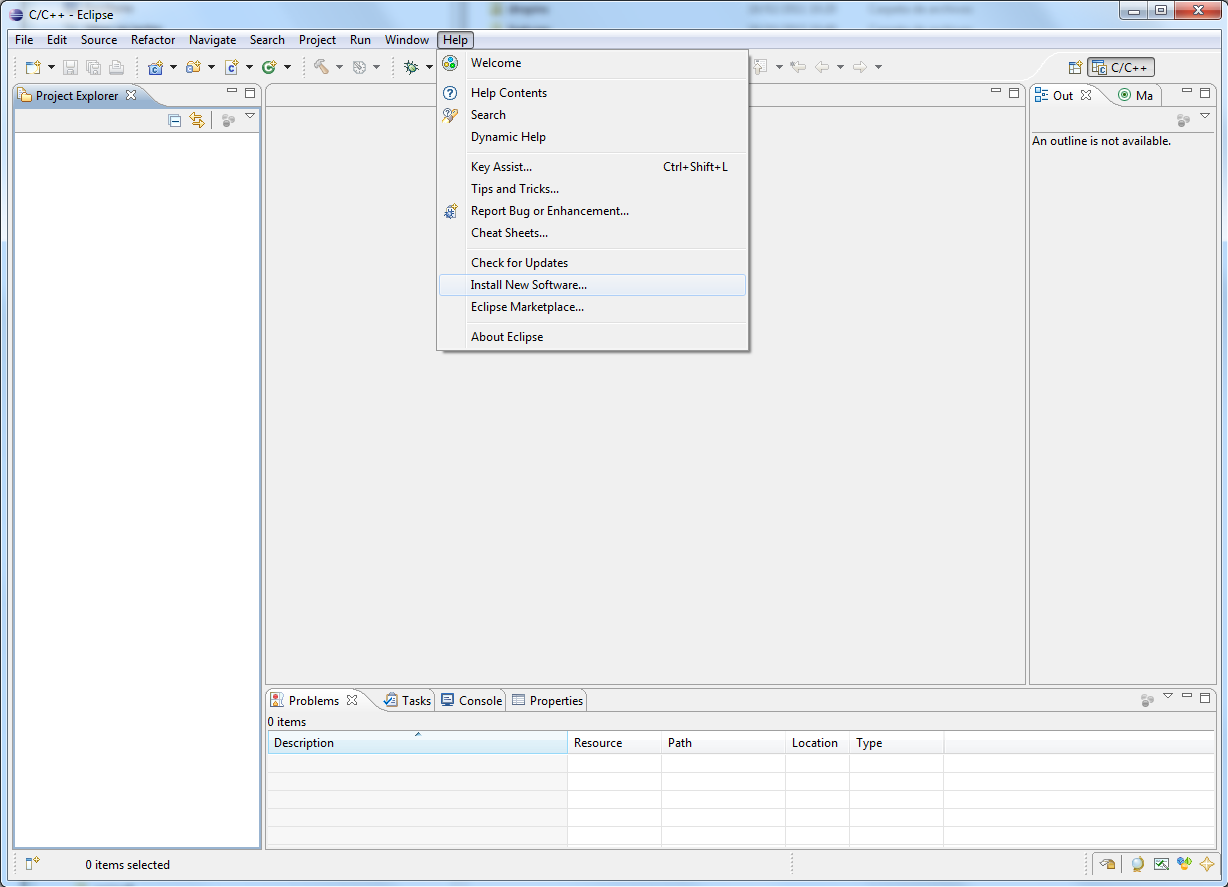
\includegraphics[height=9cm]{./Figuras/C2/c2_instalar_windows1.png}
\caption{Instalación del plugin NDS en eclipse (parte 1).}
\label{fig_c2_win1}
\end{figure}

A continuación en la ventana \textit{Available Software} se pulsa el botón \textit{Add}, y se introduce la siguiente información:
\begin{itemize}
	\item Name: \textit{NDS Manager builder}
	\item Location: \textit{http://dev.snipah.com/nds/updater}
\end{itemize}

Esta operación se refleja en la Figura \ref{fig_c2_win2}.

\begin{figure}[t]
\centering
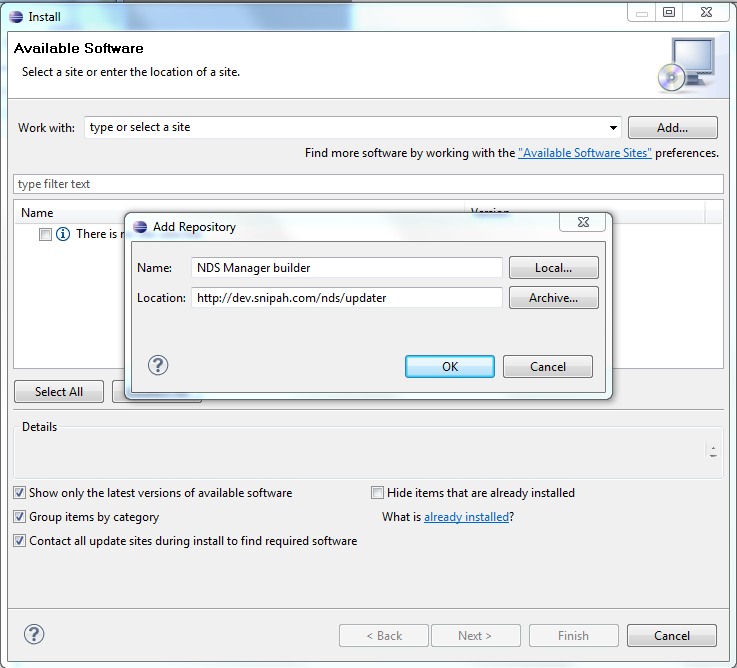
\includegraphics[height=8cm]{./Figuras/C2/c2_instalar_windows2.png}
\caption{Instalación del plugin NDS en eclipse (parte 2).}
\label{fig_c2_win2}
\end{figure}

Para que el proceso se realice de forma adecuada hay que tener la precaución de desactivar la opción \textit{Group items by category}. De esta forma aparecerá el software buscado, debiendo activarse las casillas correspondientes a \textit{devkitARM}, tal y como muestra la Figura \ref{fig_c2_win4}.

\begin{figure}[t]
\centering
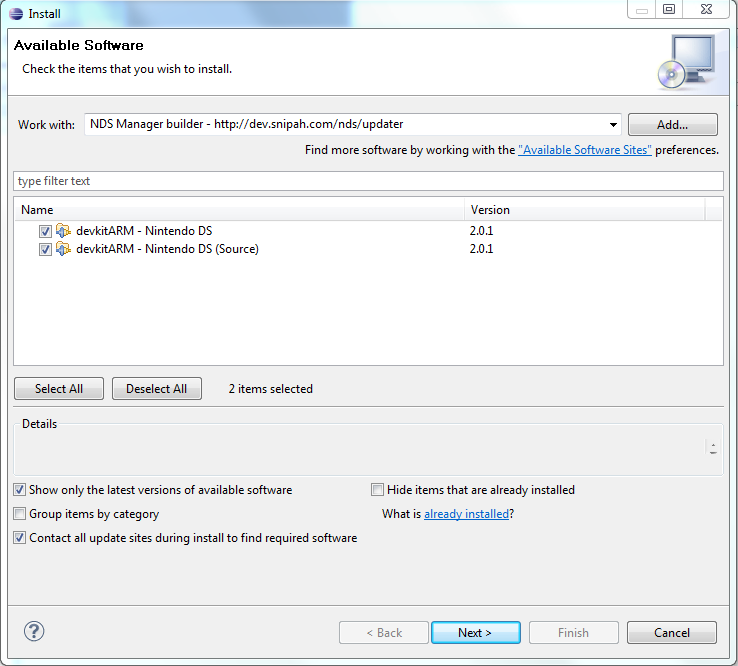
\includegraphics[height=8cm]{./Figuras/C2/c2_instalar_windows4.png}
\caption{Instalación del plugin NDS en eclipse (parte 3).}
\label{fig_c2_win4}
\end{figure}

Después de pulsar en sucesivos botones \textit{Next} y aceptar la licencia, comienza la instalación  del software. Durante dicho proceso puede aparecer la Figura \ref{fig_c2_win6}.

\begin{figure}[t]
\centering
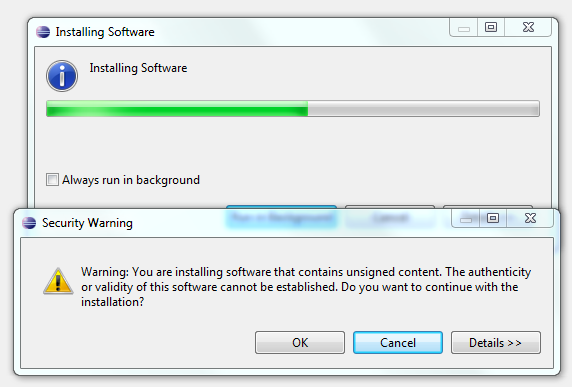
\includegraphics[height=7cm]{./Figuras/C2/c2_instalar_windows6.png}
\caption{Instalación del plugin NDS en eclipse (parte 4).}
\label{fig_c2_win6}
\end{figure}

Simplemente se pulsa en \textit{OK} para continuar el proceso de instalación. Una vez finalizada la instalación se debe reiniciar \textit{eclipse}.

Como comprobación de que todo ha ido correctamente, a la hora de crear el proyecto se debe observar que aparece algo parecido a lo mostrado en la Figura \ref{fig_c2_win7}.

\begin{figure}[h]
\centering
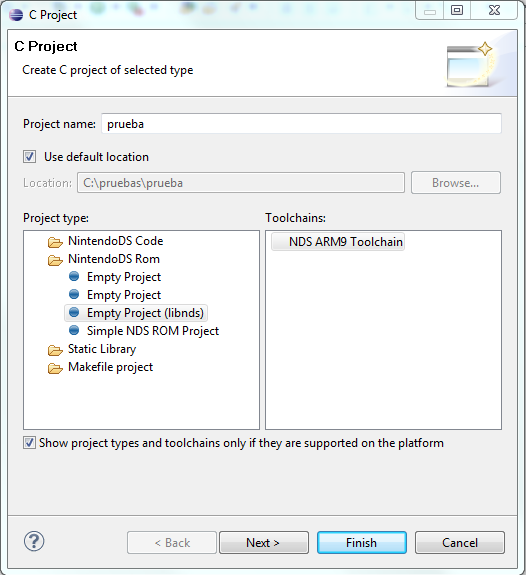
\includegraphics[height=8cm]{./Figuras/C2/c2_instalar_windows7.png}
\caption{Instalación del plugin NDS en eclipse (parte 5).}
\label{fig_c2_win7}
\end{figure}


Se elige \textit{Empty Project (libnds)}, y si después de pulsar en \textit{Next} aparece lo mostrado en la Figura \ref{fig_c2_win8}, entonces todo está correcto.

\newpage

\begin{figure}[h]
\centering
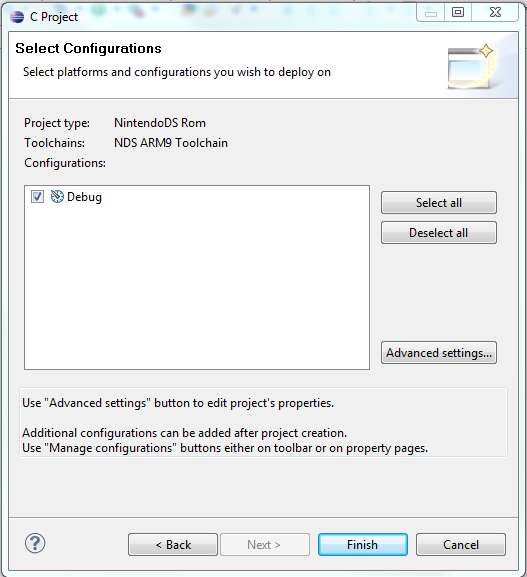
\includegraphics[height=8cm]{./Figuras/C2/c2_instalar_windows8.png}
\caption{Instalación del plugin NDS en eclipse (parte 6).}
\label{fig_c2_win8}
\end{figure}


% --------------------------------------------------------------------------
% --------------------------------------------------------------------------
% --------------------------------------------------------------------------
% --------------------------------------------------------------------------
\section{Nuestro primer programa para NDS en Windows}
En esta sección se van a ver los pasos para realizar nuestro primer programa para la NDS en el sistema operativo \textit{Windows}. 

% --------------------------------------------------------------------------
% --------------------------------------------------------------------------

\subsection{Desarrollar código para la NDS sin emplear Eclipse}
\label{sec:programa}
En este apartado se va a crear el primer programa en la NDS sin emplear \textit{Eclipse} como herramienta de desarrollo.

% --------------------------------------------------------------------------
\subsubsection{Creación de la estructura de ficheros}
Se puede emplear como punto de partida el ejemplo  \textit{hello\_world} que aparece en el directorio \textit{nds} del directorio \textit{examples} de  \textit{DevkitPro}. En  el laboratorio de prácticas, \textit{DevkitPro} se encuentra en el directorio \textit{C:$\backslash$}. En el directorio donde se vayan a almacenar los  programas a desarro\-llar se crea un nuevo directorio que identifique el programa a desarrollar (p.ej. \textit{ejemplo}). Dentro de ese directorio se crea el directorio \textit{source}, que contendrá los ficheros necesarios para el código a desarrollar (p.ej. \textit{main.c}). En el directorio \textit{ejemplo} se copia el fichero \textit{Makefile} del  ejemplo  \textit{hello\_world} de \textit{DevkitPro}. De esta forma la estructura de ficheros que se tiene es la siguiente:

{\scriptsize
 \begin{verbatim}
  c:\mis_ejemplos
    - directorio ejemplo
      - fichero Makefile
      - directorio source
      - fichero main.c
\end{verbatim}
}

% --------------------------------------------------------------------------
\subsubsection{Edición del fichero ejemplo}
Para familiarizarse con el entorno de desarrollo de aplicaciones para Nintendo DS, se va a utilizar como ejemplo una aplicación en la que aparezca un saludo con el nombre del desarrollador del programa. Para escribir este código se puede emplear cualquier editor de texto. Según esto, el código del programa a desarrollar (\textit{main.c}) es el siguiente:

\begin{lstlisting}
#include<nds.h>
#include<stdio.h>
int main(void) {
    consoleDemoInit();
    iprintf("Hola mundo");  // Imprimir el mensaje 
    while(1) {} // Bucle que no hace nada.     
}
\end{lstlisting}

En dicho código cabe destacar lo siguiente:
\begin{itemize}
\item \textit{consoleDemoInit}: inicializa una consola de texto predeterminada, sin permitir elegir la pantalla donde se imprimie el texto. En este caso, será la pantalla inferior de la videoconsola. Se verán más detalles de cómo seleccionar la pantalla en la que se visualiza información en prácticas posteriores. 
%
\item  \textit{iprintf("Hola mundo")}: esta función imprime texto con formato, soportando solo números enteros.
\end{itemize}

% --------------------------------------------------------------------------
\subsubsection{Compilación del fichero ejemplo}
El siguiente paso es compilar el programa, para ello se abre el \textit{símbolo del sistema}. Una vez se está en el directorio \textit{ejemplo} creado, se ejecuta el comando \textit{make}:

{\scriptsize
\begin{verbatim}
 C:\mis_ejemplos\ejemplo>dir
 29/07/2013  15:10    <DIR>          .
 29/07/2013  15:10    <DIR>          ..
 02/04/2012  22:02             4.903 Makefile
 29/07/2013  15:10    <DIR>          source
                1 archivos          4.903 bytes
                3 dirs  51.779.096.576 bytes libres
 \end{verbatim}
}

{\scriptsize
\begin{verbatim}
 C:\mis_ejemplos\ejemplo>make
 main.c
 arm-none-eabi-gcc -MMD -MP -MF /d/mis_ejemplos/ejemplo/build/main.d -g -Wall 
 -O2 -march=armv5te -mtune=arm946e-s -fomit-frame-pointer -ffast-ma
 th -mthumb -mthumb-interwork -I/d/mis_ejemplos/ejemplo/include
 -I/d/mis_ejemplos/ejemplo/build -I/c/devkitPro/libnds/include 
 -I/d/mis_ejemplos/ejemplo/build -DARM9 -c /d/mis_ejemplos/ejemplo/source/main.c 
 -o main.o
 linking ejemplo.elf
 Nintendo DS rom tool 1.50.1 - Jun 19 2012
 by Rafael Vuijk, Dave Murphy, Alexei Karpenko
 built ... ejemplo.nds
\end{verbatim}
}

Si no se han producido errores de compilación aparecerán los ficheros  \textit{ejemplo.elf} y \textit{ejemplo.nds}.

{\scriptsize
 \begin{verbatim}
 C:\mis_ejemplos\ejemplo>dir
 29/07/2013  15:15    <DIR>          .
 29/07/2013  15:15    <DIR>          ..
 29/07/2013  15:15    <DIR>          build
 29/07/2013  15:15           234.949 ejemplo.elf
 29/07/2013  15:15           134.208 ejemplo.nds
 02/04/2012  22:02             4.903 Makefile
 29/07/2013  15:10    <DIR>          source
                3 archivos        374.060 bytes
                4 dirs  51.778.568.192 bytes libres
 \end{verbatim}
}

El primero (\textit{ejemplo.elf}) es el que contiene la información de depuración, por tanto, el depurador tendrá que trabajar necesariamente con él. Sin embargo,  la consola (o el emulador) solo será capaz de ejecutar la imagen del cartucho \textit{ejemplo.nds}. También se ha creado el directorio \textit{build}, que por ahora no tiene interés para lo que se  se está desarrollando. Para borrar todos los ficheros y directorios creados durante la compilación se puede ejecutar \textit{make clean}.

Si se produjese un error relacionado con que no encuentra el compilador se puede realizar lo siguiente:
\begin{itemize}
\item Hacer una copia de los siguientes ficheros que se encuentran en \textit{C:$\backslash$ devkitPro $\backslash$ devkitARM $\backslash$ bin}:	
	\begin{itemize}
 		\item arm-none-eabi-as
 		\item arm-none-eabi-g++
	 	\item arm-none-eabi-gcc	
 		\item arm-none-eabi-gdb
	   \item arm-none-eabi-objcopy
	\end{itemize}
\item Renombrar las copias con los siguientes nombres:	
	\begin{itemize}
		\item arm-eabi-as
	 	\item arm-eabi-g++
	 	\item arm-eabi-gcc	
 		\item arm-eabi-gdb
	   \item arm-eabi-objcopy
	\end{itemize}
\end{itemize}

% --------------------------------------------------------------------------
\subsubsection{Ejecución del fichero ejemplo en el emulador}
Si no se ha producido ningún problema en la compilación, la salida del programa se puede ver en el emulador. Una vez abierto \textit{WinDS Pro}, si se escoge el emulador \textit{No\$gba}, se pulsa en \textit{File->Cartridge Menu (File Name)} y se busca el fichero \textit{.nds} que nos interesa. En nuestro caso, y una vez elegido \textit{ejemplo.nds} aparece la ventana en el emulador mostrada en la Figura \ref{fig_c2_eclipse11b}.

\begin{figure}[h]
\centering
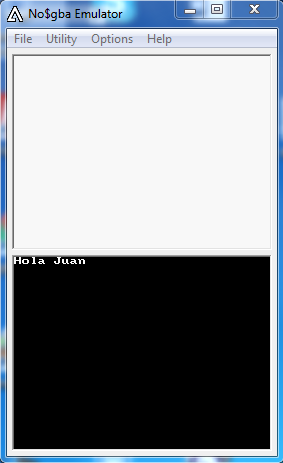
\includegraphics[height=8cm]{./Figuras/C2/c2_eclipse11b.png}
\caption{Ejecución del programa ejemplo en el emulador \textit{No\$gba}.}
\label{fig_c2_eclipse11b}
\end{figure}

Si se escoge el emulador \textit{DeSmuME}, se pulsa en \textit{File->Open ROM} y se busca el fichero \textit{.nds} que nos interesa.

% --------------------------------------------------------------------------
% --------------------------------------------------------------------------
\subsection{Desarrollar código para la NDS empleando Eclipse}
\label{sin_eclipse}
En este apartado se va a crear el primer programa en la NDS empleando \textit{Eclipse} como herramienta de desarrollo.

% --------------------------------------------------------------------------
\subsubsection{Creación de un proyecto para NDS}
En  el laboratorio de prácticas, \textit{Eclipse} se encuentra en el directorio \textit{C:$\backslash$}. Al iniciar \textit{Eclipse} se pide el directorio donde se almacenará el proyecto a crear, tal como muestra la Figura \ref{fig_c2_eclipse1}.

\begin{figure}[t]
\centering
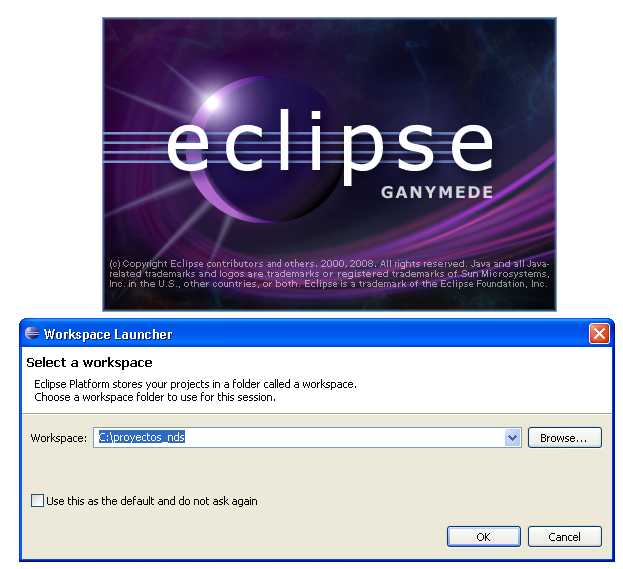
\includegraphics[height=9cm]{./Figuras/C2/c2_eclipse1.png}
\caption{Creación de un proyecto para NDS usando Eclipse (parte 1).}
\label{fig_c2_eclipse1}
\end{figure}


Para crear un nuevo proyecto se debe pulsar en la ventana principal de \textit{Eclipse} en \textit{File->New->C project} (ver Figura \ref{fig_c2_eclipse2}). 

\begin{figure}[t]
\centering
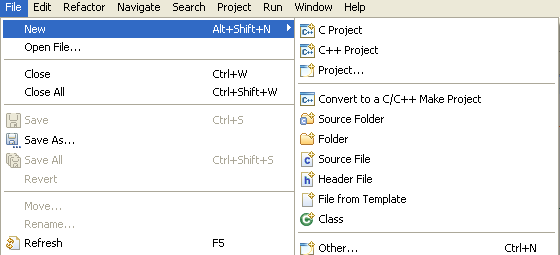
\includegraphics[height=6cm]{./Figuras/C2/c2_eclipse2.png}
\caption{Creación de un proyecto para NDS usando Eclipse (parte 2).}
\label{fig_c2_eclipse2}
\end{figure}

Aparece la ventana (\textit{C Project}) mostrada en la Figura \ref{fig_c2_eclipse3}.

\begin{figure}[t]
\centering
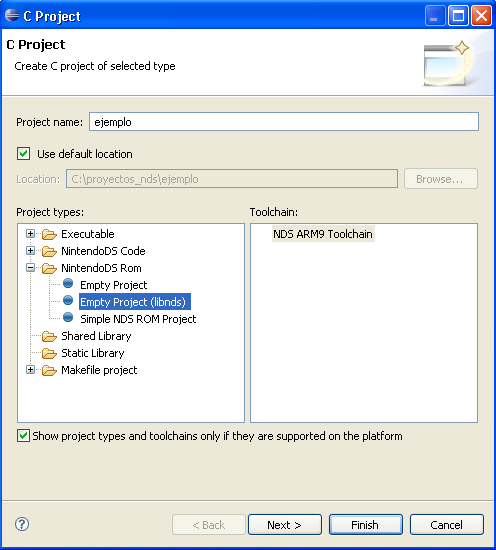
\includegraphics[height=8cm]{./Figuras/C2/c2_eclipse3.png}
\caption{Creación de un proyecto para NDS usando Eclipse (parte 3).}
\label{fig_c2_eclipse3}
 \end{figure}

\noindent en la que se debe configurar lo siguiente:
\begin{itemize}
\item El nombre del proyecto (p.ej. \textit{ejemplo}).
\item En \textit{Project types} se selecciona \textit{Nintendo DS Rom-> Empty Project (libnds)}.
\item Se pulsa en \textit{Next}.
\end{itemize}

Aparece una ventana de \textit{Select Configurations} en la que se pulsa en \textit{Finish}. 

Una vez creado el proyecto, si lo que aparece es la siguiente ventana se debe elegir el icono de \textit{workbench}, tal y como se muestra en la Figura \ref{fig_c2_eclipsew}.

\begin{figure}[t]
\centering
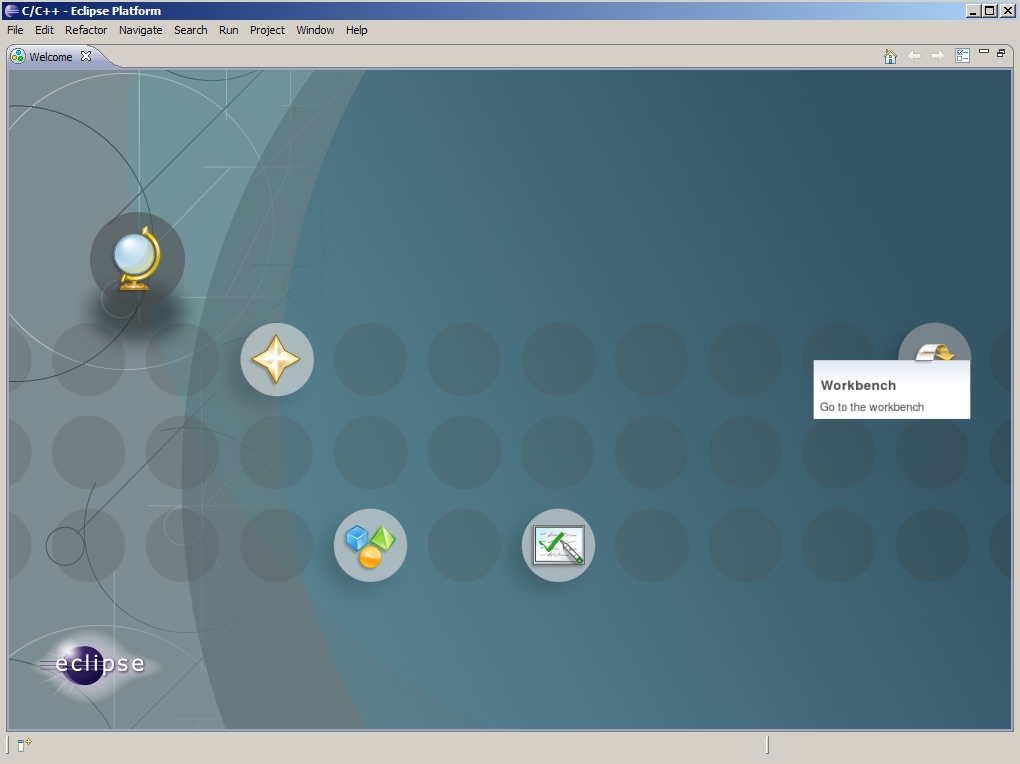
\includegraphics[height=8cm]{./Figuras/C2/c2_eclipse-workbench.png}
\caption{Creación de un proyecto para NDS usando Eclipse  (parte 4).}
\label{fig_c2_eclipsew}
\end{figure}

De esta forma, el  proyecto creado aparecerá en la ventana de \textit{workbench} de \textit{Eclipse} (ver Figura \ref{fig_c2_eclipse4}).

\begin{figure}[t]
\centering
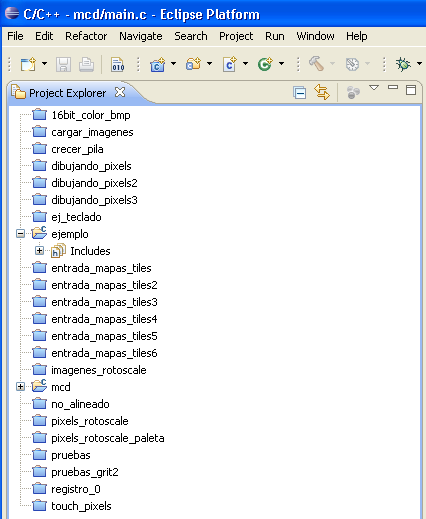
\includegraphics[height=8cm]{./Figuras/C2/c2_eclipse4.png}
\caption{Creación de un proyecto para NDS usando Eclipse (parte 5).}
\label{fig_c2_eclipse4}
\end{figure}

Esta ventana podría aparecer directamente sin necesidad de elegir el icono de \textit{workbench} de \textit{Eclipse}.

% --------------------------------------------------------------------------
\subsubsection{Configuración del proyecto}
Para iniciar la configuración del proyecto, se debe pulsar en la ventana principal de \textit{Eclipse} en \textit{Project Properties}, teniendo la precaución de tener activado el proyecto que se desea. Una vez realizada esta operación aparece la ventana (\textit{Properties for ejemplo}) (ver Figura \ref{fig_c2_eclipse5}).

\begin{figure}[t]
\centering
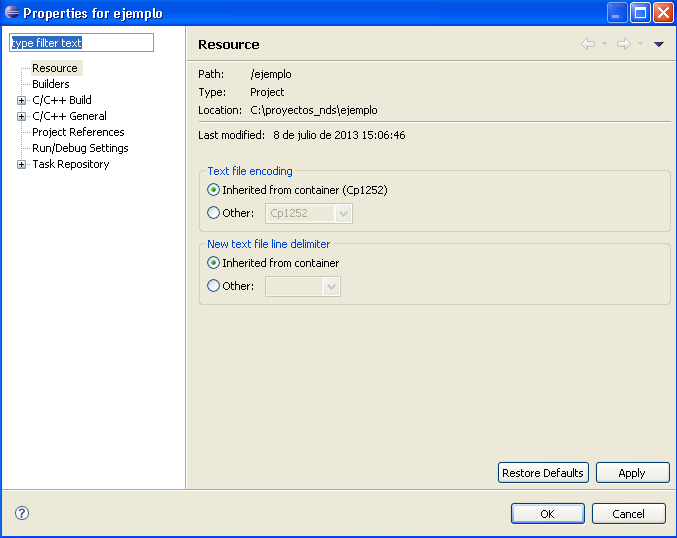
\includegraphics[height=8cm]{./Figuras/C2/c2_eclipse5.png}
\caption{Creación de un proyecto para NDS usando Eclipse (parte 6).}
\label{fig_c2_eclipse5}
\end{figure}

En dicha ventana se debe desplegar la pestaña \textit{C/C++ Build}. Se resalta dicha opción. En el cuadro \textit{Builder} de la pestaña \textit{Builder Settings} se cambia la opción \textit{Builder Type} a \textit{Internal Builder} (ver Figura \ref{fig_c2_eclipse6}).

\begin{figure}[t]
	\centering
	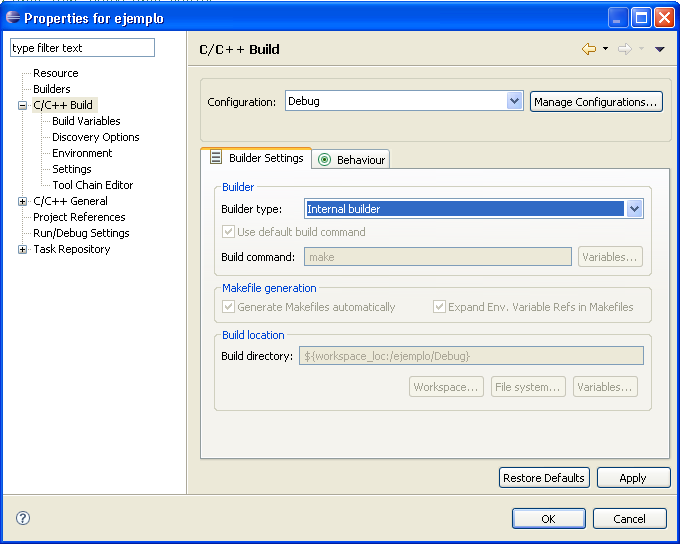
\includegraphics[height=8cm]{./Figuras/C2/c2_eclipse6.png}
	\caption{Creación de un proyecto para NDS usando Eclipse (parte 7).}
	\label{fig_c2_eclipse6}
\end{figure}

En la pestaña \textit{C/C++ Build} se resalta \textit{Settings}, apareciendo la ventana que se muestra en la Figura \ref{fig_c2_eclipse7}.

\begin{figure}[t]
	\centering
	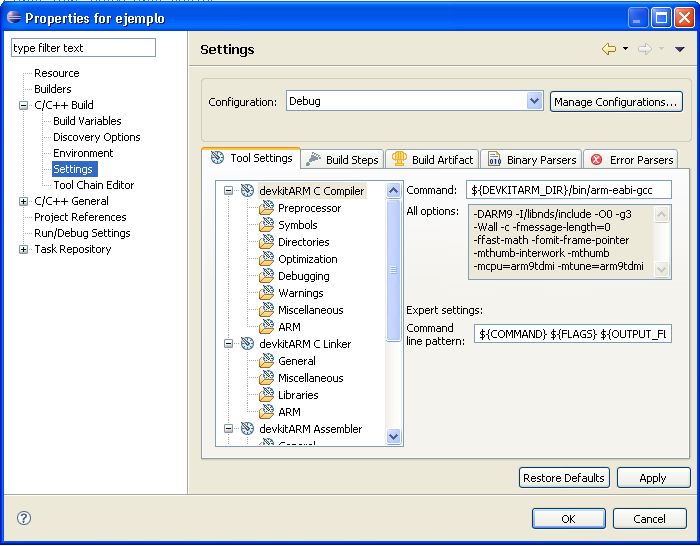
\includegraphics[height=8cm]{./Figuras/C2/c2_eclipse7.png}
	\caption{Creación de un proyecto para NDS usando Eclipse  (parte 8).}
	\label{fig_c2_eclipse7}
\end{figure}

Se escoge \textit{devkitARM C Linker->ARM} y se desactiva la opción \textit{No FPU}. Finalmente se pulsa en \textit{OK} (ver Figura \ref{fig_c2_eclipse8}).

\begin{figure}[t]
	\centering
	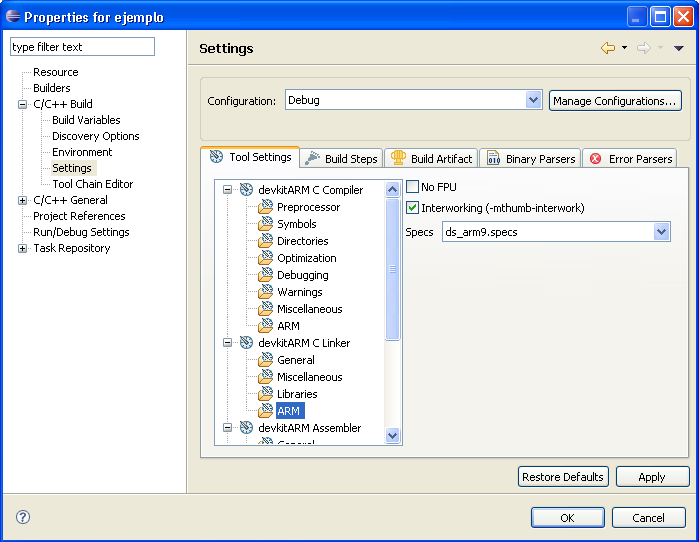
\includegraphics[height=8cm]{./Figuras/C2/c2_eclipse8.png}
	\caption{Creación de un proyecto para NDS usando Eclipse  (parte 9).}
	\label{fig_c2_eclipse8}
\end{figure}

% --------------------------------------------------------------------------
\subsubsection{Edición del fichero ejemplo}
Para familiarizarse con el entorno de desarrollo de \textit{Eclipse} para NDS, se utiliza el mismo ejemplo que el del apartado anterior. En primer lugar, se debe crear un fichero fuente en \textit{lenguaje C} dentro del proyecto actual. Para ello se pulsa en \textit{File->New->Source File} (ver Figura \ref{fig_c2_eclipse9}).

\begin{figure}[t]
	\centering
	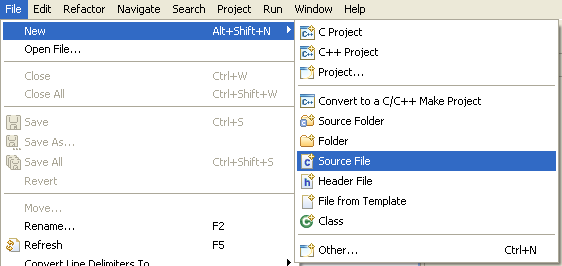
\includegraphics[height=7cm]{./Figuras/C2/c2_eclipse9.png}
	\caption{Creación de un proyecto para NDS usando Eclipse  (parte 10).}
	\label{fig_c2_eclipse9}
\end{figure}

Aparece una nueva ventana (\textit{New Source File}) (ver Figura \ref{fig_c2_eclipse10}).

\begin{figure}[t]
	\centering
	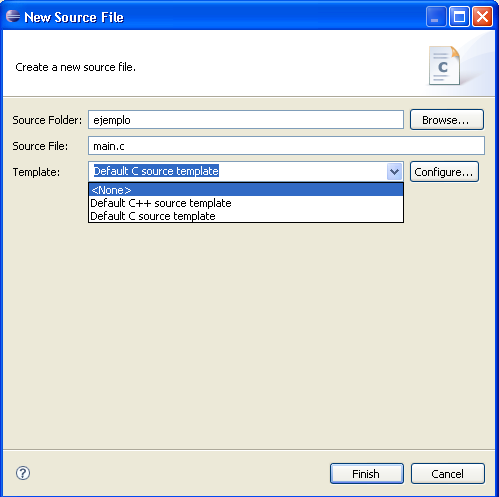
\includegraphics[height=7cm]{./Figuras/C2/c2_eclipse10.png}
	\caption{Creación de un proyecto para NDS usando Eclipse  (parte 11).}
	\label{fig_c2_eclipse10}
\end{figure}


\noindent en la que se debe realizar lo siguiente:
\begin{itemize}
 	\item En \textit{Source File} se introduce \textit{main.c}.
 	\item En \textit{Template} se selecciona \textit{None}.
 	\item Se pulsa en \textit{Finish}.
\end{itemize}

A continuación en la ventana que hace referencia a \textit{main.c} se introduce el mismo código que el del apartado \ref{sec:programa}.

% --------------------------------------------------------------------------
\subsubsection{Compilación del fichero ejemplo}
El siguiente paso es compilar el programa, para ello se elige \textit{Project->Build Project}. Si no se han producido errores de compilación aparecerán los ficheros  \textit{ejemplo.elf} y \textit{ejemplo.nds} en el directorio \textit{Debug}, tal y como se puede comprobar en la Figura \ref{fig_c2_ficheros_eclipse}.

\begin{figure}[t]
	\centering
	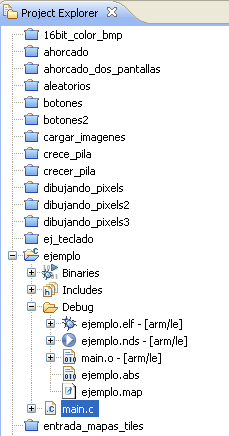
\includegraphics[height=7cm]{./Figuras/C2/c2_ficheros_eclipse.png}
	\caption{Creación de un proyecto para NDS usando Eclipse  (parte 12).}
	\label{fig_c2_ficheros_eclipse}
\end{figure}

Si se produjese un error relacionado con que no encuentra el compilador se puede realizar lo siguiente:
\begin{itemize}
\item Hacer una copia de los siguientes ficheros que se encuentran en \textit{C:$\backslash$ devkitPro $\backslash$ devkitARM $\backslash$ bin}:	
	\begin{itemize}
	 	\item arm-none-eabi-as
	 	\item arm-none-eabi-g++
	 	\item arm-none-eabi-gcc	
	 	\item arm-none-eabi-gdb
	   \item arm-none-eabi-objcopy
	\end{itemize}
\item Renombrar las copias con los siguientes nombres:	
	\begin{itemize}
	 	\item arm-eabi-as
	 	\item arm-eabi-g++
	 	\item arm-eabi-gcc	
	 	\item arm-eabi-gdb
	   \item arm-eabi-objcopy
	 \end{itemize}
\end{itemize}


% --------------------------------------------------------------------------
\subsubsection{Ejecución del fichero ejemplo en el emulador}
Una vez abierto \textit{WinDS Pro}, si se escoge el emulador \textit{No\$gba}, se pulsa en \textit{File->Cartridge Menu (File Name)} y se busca el fichero \textit{.nds} que nos interesa. En nuestro caso, y una vez elegido \textit{ejemplo.nds} aparece la ventana en el emulador mostrada en la Figura \ref{fig_c2_eclipse11b}.

Si se escoge el emulador \textit{DeSmuME}, se pulsa en \textit{File->Open ROM} y se busca el fichero \textit{.nds} que nos interesa.

% --------------------------------------------------------------------------
% --------------------------------------------------------------------------
% --------------------------------------------------------------------------
% --------------------------------------------------------------------------
\section{Instalación del entorno de desarrollo en Linux}
Las operaciones a seguir para instalar el entorno de desarrollo en Linux son las siguientes:

\begin{enumerate}
\item Instalación de \textit{devkitpro}. Se accede a la página web:
 	\begin{verbatim}
 	http://devkitpro.org/
 	\end{verbatim}
Se pulsa en \textit{For instructions on installing the toolchains see our Getting Started pages} y posteriormente elegir \textit{Manual instructions for installing devkitARM} y seguir los pasos que aparecen en dicha página web.
%	
\item Instalación de \textit{WinDS Pro}. Se puede descargar la última versión de \textit{WinDS Pro} de la siguiente página web:
	\begin{verbatim}
	 https://windsprocentral.blogspot.com.es/2016/10/winds-pro.html
	\end{verbatim} 
%
\item Instalación de \textit{desmume}. Se pueden seguir los pasos que aparecen en la siguiente página web:
{\scriptsize
	\begin{verbatim}
		http://wiki.desmume.org/index.php?title=Installing_DeSmuME_from_source_on_Linux
	\end{verbatim}
}

Recomendable emplear la opción \textit{Install desmume from svn}.
%
\item Instalación de \textit{eclipse} \textit{Helios}. Se siguen los mismos pasos que los indicados para Windows.
%
\item Instalación del \textit{plugin NDS ManagedBuilder}. En este caso será necesario  instalar el plugin mediante el actualizador del propio Eclipse que se encuentra en \textit{Help->Install New Software}. Para ello se emplea la \textit{url} de actualizaciones del \textit{NDS Managed builder}
 \textit{(http://dev.snipah.com/nds/updater)}, que se deberá especificar en la ventana mostrada en la Figura \ref{fig_c2_managebuilder}.
\end{enumerate}

\begin{figure}[t]
	\centering
	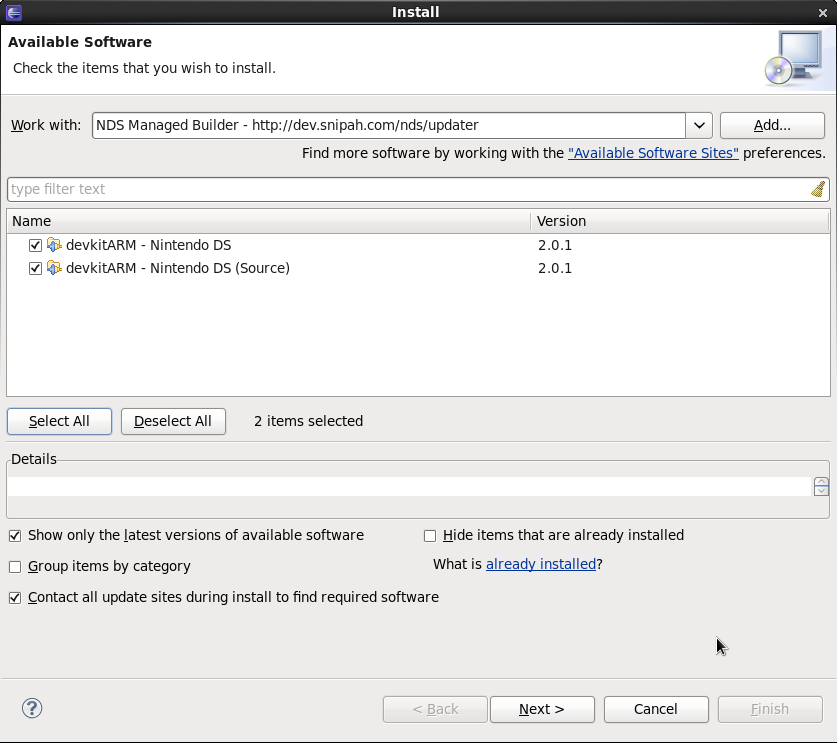
\includegraphics[height=8cm]{./Figuras/C2/c2_Pantallazo2.png}
	\caption{Instalación del \textit{plugin NDS ManagedBuilder}}
	\label{fig_c2_managebuilder}
\end{figure}


Hay que tener la precaución de desactivar la opción \textit{Group items by category}. Después de aceptar la licencia se instalará el plugin. Una vez finalizada la instalación se debe reiniciar Eclipse.

% --------------------------------------------------------------------------
% --------------------------------------------------------------------------
\section{Nuestro primer programa para NDS en Linux}
En esta sección se van a ver los pasos para realizar nuestro primer programa para la NDS en el sistema operativo \textit{Linux}. \textbf{En el laboratorio se debe entrar con la cuenta \textit{usuario}}. Antes de nada se debe comprobar que las siguientes variables de entorno se encuentran en el fichero \textit{.bash\_profile} del \textit{usuario}:
\begin{verbatim}
 export DEVKITPRO=/opt/devkitpro/
 export DEVKITARM=/opt/devkitpro/devkitARM/
\end{verbatim}

% --------------------------------------------------------------------------
% --------------------------------------------------------------------------
\subsection{Desarrollar código para la NDS sin emplear Eclipse}
En este apartado se va a crear el primer programa en la NDS sin emplear \textit{Eclipse} como herramienta de desarrollo.

% --------------------------------------------------------------------------
\subsubsection{Creación de la estructura de ficheros}
Se puede emplear como punto de partida el ejemplo  \textit{hello\_world} que aparece en el directorio \textit{nds} del directorio \textit{examples} de  \textit{DevkitPro}. En  el laboratorio de prácticas, \textit{DevkitPro} se encuentra en el directorio \textit{/opt/devkitpro}. En el directorio donde se vayan a almacenar los programas a desarro\-llar se crea un nuevo directorio que identifique el programa a desarrollar (p.ej. \textit{ejemplo}). Dentro de ese directorio se crea el directorio \textit{source}, que contendrá los ficheros necesarios para el código a desarrollar (p.ej. \textit{main.c}). En el directorio \textit{ejemplo} se copia el fichero \textit{Makefile} del  ejemplo  \textit{hello\_world} de \textit{DevkitPro}. De esta forma la estructura de ficheros que se tiene es la siguiente:
\begin{verbatim}
  /home/usuario/mis_ejemplos
    - directorio ejemplo
      - fichero Makefile
      - directorio source
      - fichero main.c
\end{verbatim}



% --------------------------------------------------------------------------
\subsubsection{Edición del fichero ejemplo}
Para familiarizarse con el entorno de desarrollo de aplicaciones para Nintendo DS, se va a utilizar como ejemplo una aplicación en la que aparezca un saludo con el nombre del desarrollador del programa. Para escribir este código se puede emplear cualquier editor de texto.

Según esto, el código del programa a desarrollar (\textit{main.c}) es el siguiente:
\begin{lstlisting}
#include<nds.h>
#include<stdio.h>
int main(void)
{
	consoleDemoInit();
    iprintf("Hola Juan");  // Imprimir el mensaje 
    while(1){} // Bucle que no hace nada.     
    return 0; // Finalizar el programa
}
\end{lstlisting}

% --------------------------------------------------------------------------
\subsubsection{Compilación del fichero ejemplo}
El siguiente paso es compilar el programa, para ello se abre el \textit{Terminal} \textit{(Sistema->Terminal)}. Una vez se está en el directorio \textit{ejemplo} creado, se ejecuta el comando \textit{make}:
\begin{verbatim}
 [usuario@labsop02 ejemplo]# make
 main.c
 arm-none-eabi-gcc -MMD -MP -MF /root/mis_ejemplos/ejemplo/build/main.d -g -Wall 
 -O2 -march=armv5te -mtune=arm946e-s -fomit-frame-pointer -ffast-math 
 -mthumb -mthumb-interwork -I/root/mis_ejemplos/ejemplo/include 
 -I/root/mis_ejemplos/ejemplo/build -I/opt/devkitpro//libnds/include 
 -I/root/mis_ejemplos/ejemplo/build -DARM9 -c 
 /root/mis_ejemplos/ejemplo/source/main.c -o main.o 
 linking ejemplo.elf
 Nintendo DS rom tool 1.50.1 - Jun 19 2012
 by Rafael Vuijk, Dave Murphy, Alexei Karpenko
 built ... ejemplo.nds
\end{verbatim}

Si no se han producido errores de compilación aparecerán los ficheros \textit{ejemplo.elf} y \textit{ejemplo.nds}.
\begin{verbatim}
 [usuario@labsop02 ejemplo]# ls -l
 total 332
 drwxr-xr-x 2 root root   4096 sep  5 18:01 build
 -rwxr-xr-x 1 root root 234909 sep  5 18:01 ejemplo.elf
 -rw-r--r-- 1 root root 134208 sep  5 18:01 ejemplo.nds
 -rwxr-xr-x 1 root root   4903 abr  2  2012 Makefile
 drwxr-xr-x 2 root root   4096 sep  5 18:00 source
                \end{verbatim}
Para borrar todos los ficheros y directorios creados durante la compilación se puede ejecutar \textit{make clean}.

Si se produjese un error relacionado con que no encuentra el compilador se puede realizar lo siguiente:
\begin{itemize}
\item Hacer una copia de los siguientes ficheros que se encuentran en \textit{/opt/devkitpro/devkitARM/bin}:	
	\begin{itemize}
 	\item arm-none-eabi-as
 	\item arm-none-eabi-g++
 	\item arm-none-eabi-gcc	
 	\item arm-none-eabi-gdb
    \item arm-none-eabi-objcopy
	\end{itemize}
\item Renombrar las copias con los siguientes nombres:	
	\begin{itemize}
 	\item arm-eabi-as
 	\item arm-eabi-g++
 	\item arm-eabi-gcc	
 	\item arm-eabi-gdb
    \item arm-eabi-objcopy
    \end{itemize}
\end{itemize}

% --------------------------------------------------------------------------
\subsubsection{Ejecución del fichero ejemplo en el emulador}
Si no se ha producido ningún problema en la compilación, la salida del programa se puede ver en el emulador. Una vez abierto \textit{WinDS Pro}, si se escoge el emulador \textit{No\$gba}, se pulsa en \textit{File->Cartridge Menu (File Name)} y se busca el fichero \textit{.nds} que nos interesa. Si se escoge el emulador \textit{DeSmuME}, se pulsa en \textit{File->Open ROM} y se busca el fichero \textit{.nds} que nos interesa.


% --------------------------------------------------------------------------
% --------------------------------------------------------------------------
\subsection{Desarrollar código para la NDS empleando Eclipse}
En este apartado se va a crear el primer programa en la NDS empleando \textit{Eclipse} como herramienta de desarrollo.

% --------------------------------------------------------------------------
\subsubsection{Creación de un proyecto para NDS}
En  el laboratorio de prácticas, \textit{Eclipse} se encuentra en el directorio \textit{/opt/eclipse-helios}.  Al iniciar \textit{Eclipse} se pide el directorio donde se almacenará el proyecto a crear (ver Figura \ref{fig_pig_p3_c1_eclipel1}).

\begin{figure}[t]
\centering
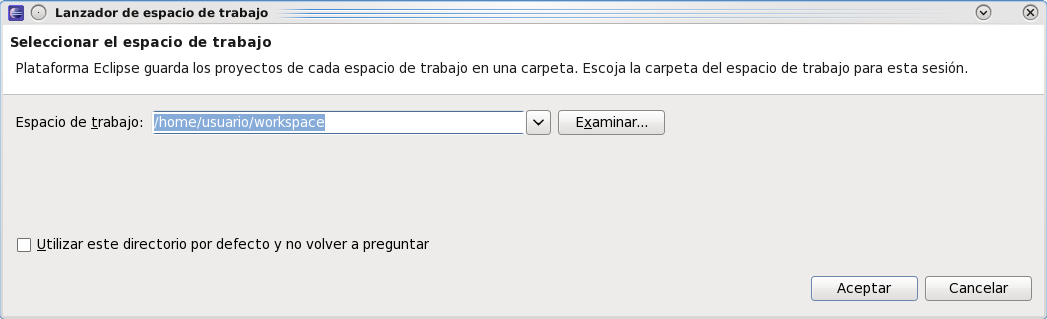
\includegraphics[height=4cm]{./Figuras/C2/c2_instan1.png}
\caption{Creación de un proyecto para NDS usando Eclipse en Linux (parte 1).}
\label{fig_pig_p3_c1_eclipel1}
 \end{figure}


Para crear un nuevo proyecto se debe pulsar en la ventana principal de \textit{Eclipse} en \textit{Archivo->Nuevo->Proyecto}.  Aparece la ventana (\textit{Proyecto nuevo}) mostrada en la Figura \ref{fig_pig_p3_c1_eclipel2}.

\begin{figure}[t]
	\centering
	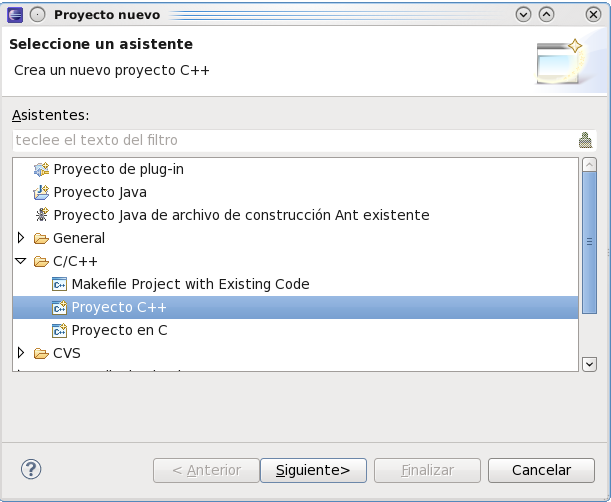
\includegraphics[height=8cm]{./Figuras/C2/c2_instan2.png}
	\caption{Creación de un proyecto para NDS usando Eclipse en Linux (parte 2).}
	\label{fig_pig_p3_c1_eclipel2}
\end{figure}

Se escoge \textit{C/C++->Proyecto en C} y se pulsa en \textit{Siguiente}, apareciendo la ventana \textit{Proyecto C} mostrada en la Figura \ref{fig_pig_p3_c1_eclipel3}.

\begin{figure}[t]
	\centering
	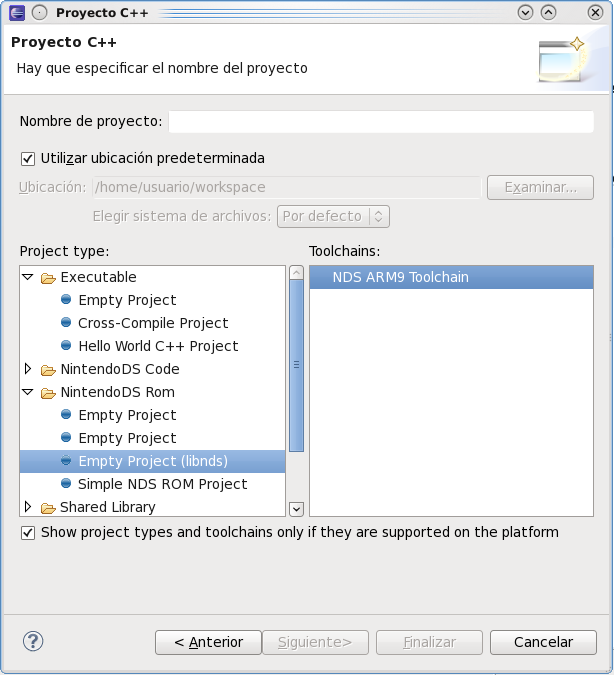
\includegraphics[height=8cm]{./Figuras/C2/c2_instan3.png}
	\caption{Creación de un proyecto para NDS usando Eclipse en Linux (parte 3).}
	\label{fig_pig_p3_c1_eclipel3}
\end{figure}

En dicha ventana se debe configurar lo siguiente:
 \begin{itemize}
 	\item El nombre de proyecto (p.ej. \textit{ejemplo}).
 	\item En \textit{Project type} se selecciona \textit{NintendoDS Rom-> Empty Project (libnds)}.
 	\item Se pulsa en \textit{Siguiente}.
 \end{itemize}

Aparece una ventana de \textit{Select Configurations} en la que se pulsa en \textit{Finalizar}. 

De esta forma, el  proyecto creado aparecerá en la ventana de \textit{workbench} de \textit{Eclipse}, lo que se muestra en la Figura \ref{fig_pig_p3_c1_eclipel4}.

\begin{figure}[t]
	\centering
	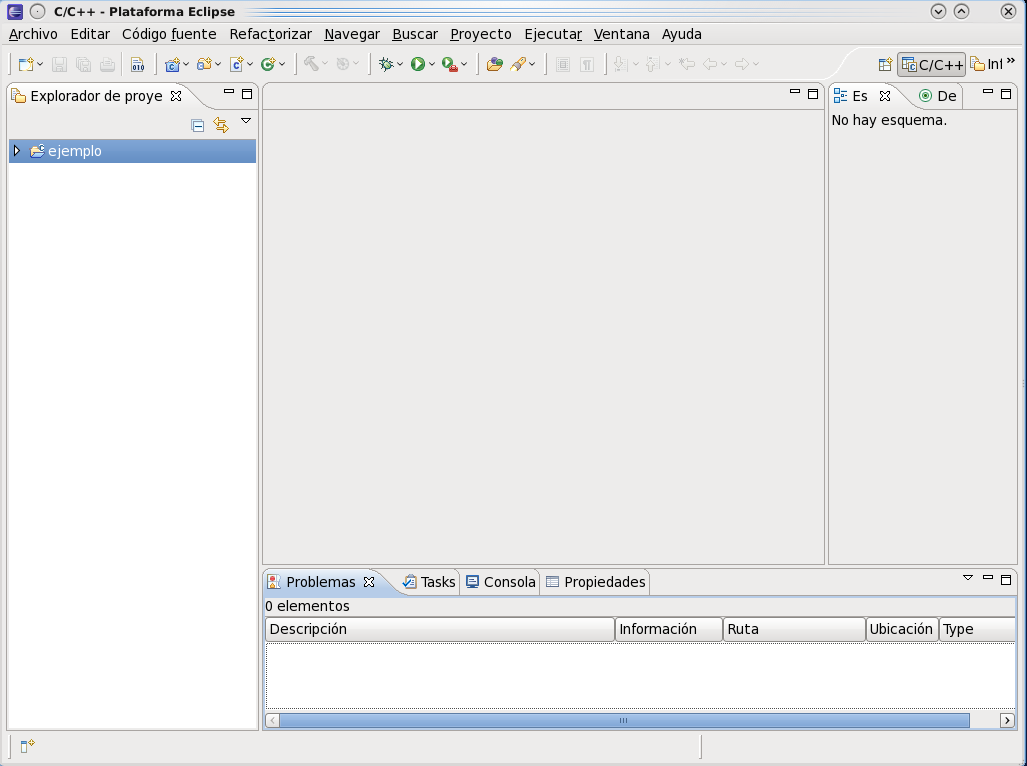
\includegraphics[height=8cm]{./Figuras/C2/c2_instan4.png}
	\caption{Creación de un proyecto para NDS usando Eclipse en Linux (parte 4).}
	\label{fig_pig_p3_c1_eclipel4}
\end{figure}

% --------------------------------------------------------------------------
\subsubsection{Configuración del proyecto}
Para iniciar la configuración del proyecto, se debe pulsar en la ventana principal de \textit{Eclipse} en \textit{Proyecto->Propiedades}, teniendo la precaución de tener activado el proyecto que se desea. Una vez realizada esta operación aparece la ventana (\textit{Propiedades de ejemplo}) (ver Figura \ref{fig_pig_p3_c1_eclipel5}).

\begin{figure}[t]
	\centering
	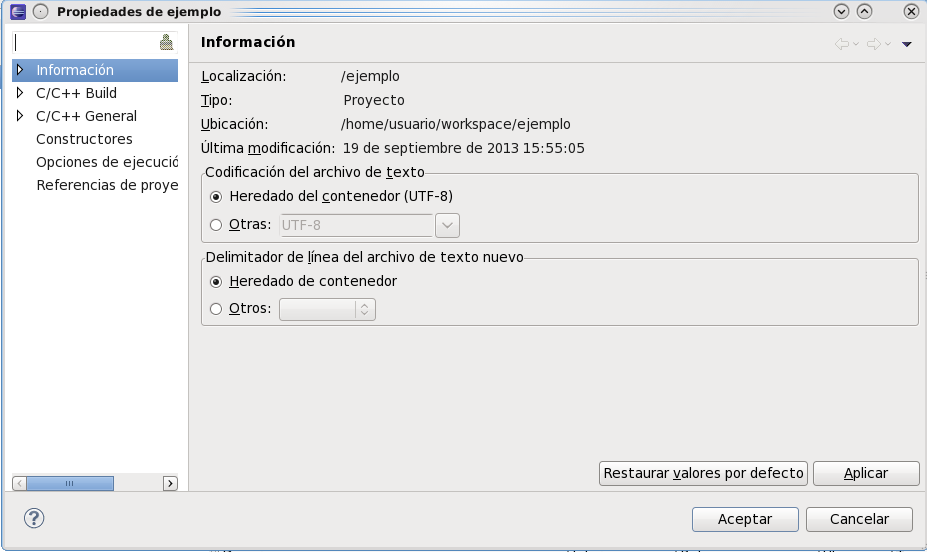
\includegraphics[height=8cm]{./Figuras/C2/c2_instan5.png}
	\caption{Creación de un proyecto para NDS usando Eclipse en Linux (parte 5).}
	\label{fig_pig_p3_c1_eclipel5}
\end{figure}

En dicha ventana se debe desplegar la pestaña \textit{C/C++ Build}. Se resalta dicha opción. En el cuadro \textit{Constructor} de la pestaña \textit{Builder Settings} se cambia la opción \textit{Builder Type} a \textit{Internal Builder} (ver Figura \ref{fig_pig_p3_c1_eclipel6}).


\begin{figure}[t]
	\centering
	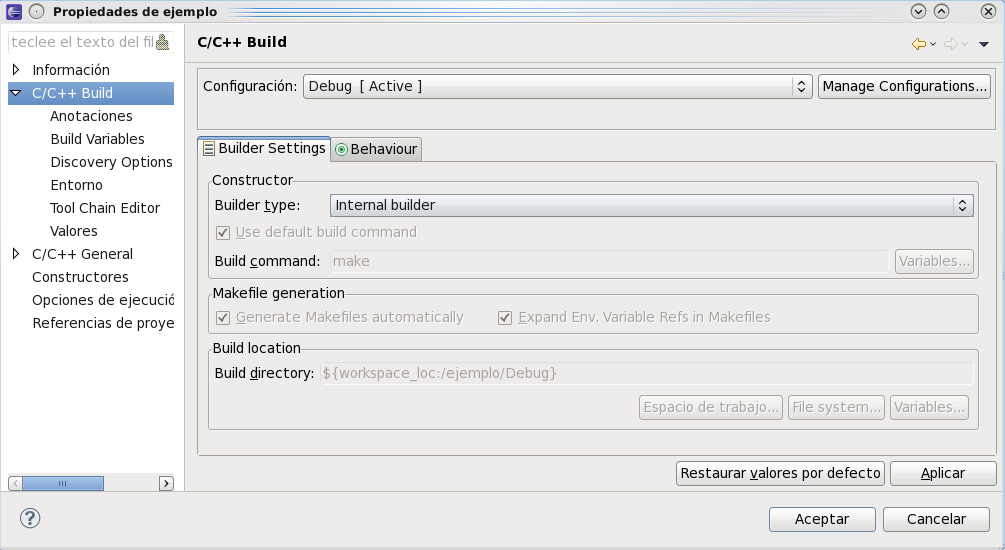
\includegraphics[height=8cm]{./Figuras/C2/c2_instan6.png}
	\caption{Creación de un proyecto para NDS usando Eclipse en Linux (parte 6).}
	\label{fig_pig_p3_c1_eclipel6}
\end{figure}

En la pestaña \textit{C/C++ Build} se resalta \textit{Valores}, apareciendo la ventana mostrada en la Figura \ref{fig_pig_p3_c1_eclipel7}.


\begin{figure}[t]
	\centering
	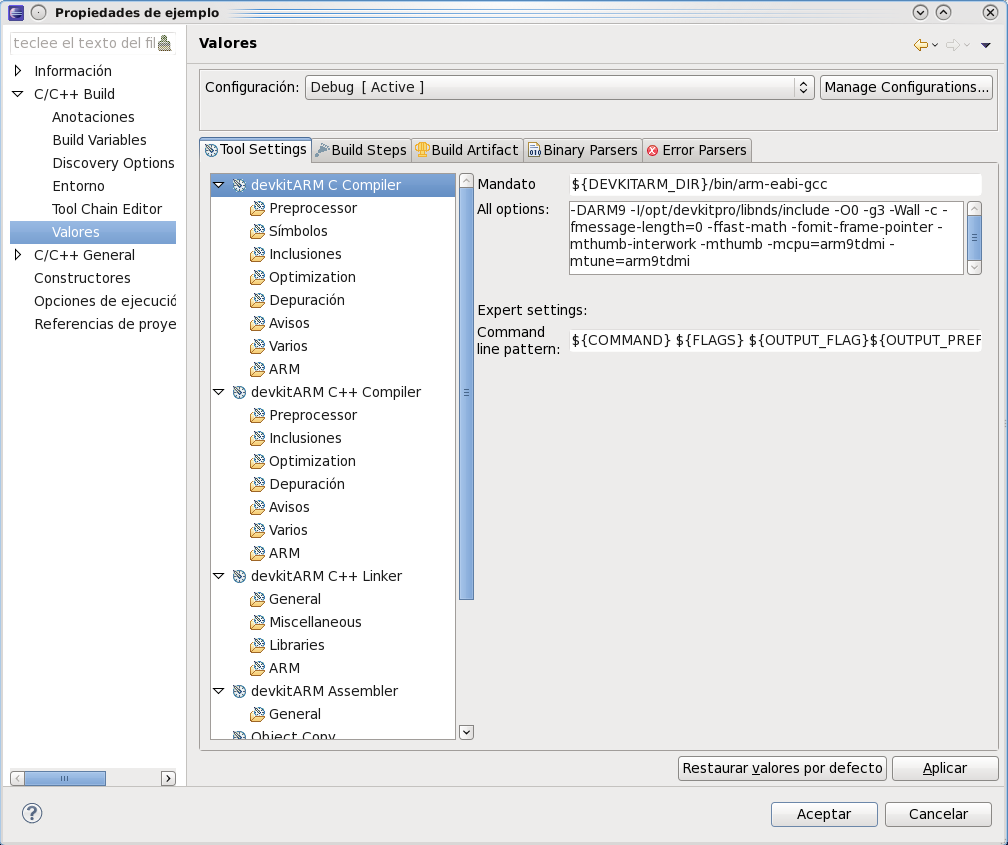
\includegraphics[height=7cm]{./Figuras/C2/c2_instan7.png}
	\caption{Creación de un proyecto para NDS usando Eclipse en Linux (parte 7).}
	\label{fig_pig_p3_c1_eclipel7}
\end{figure}

Se escoge \textit{devkitARM C Linker->ARM} y se desactiva la opción \textit{No FPU}. Finalmente se pulsa en \textit{Aceptar} (ver Figura \ref{fig_pig_p3_c1_eclipel8}).

\begin{figure}[t]
	\centering
	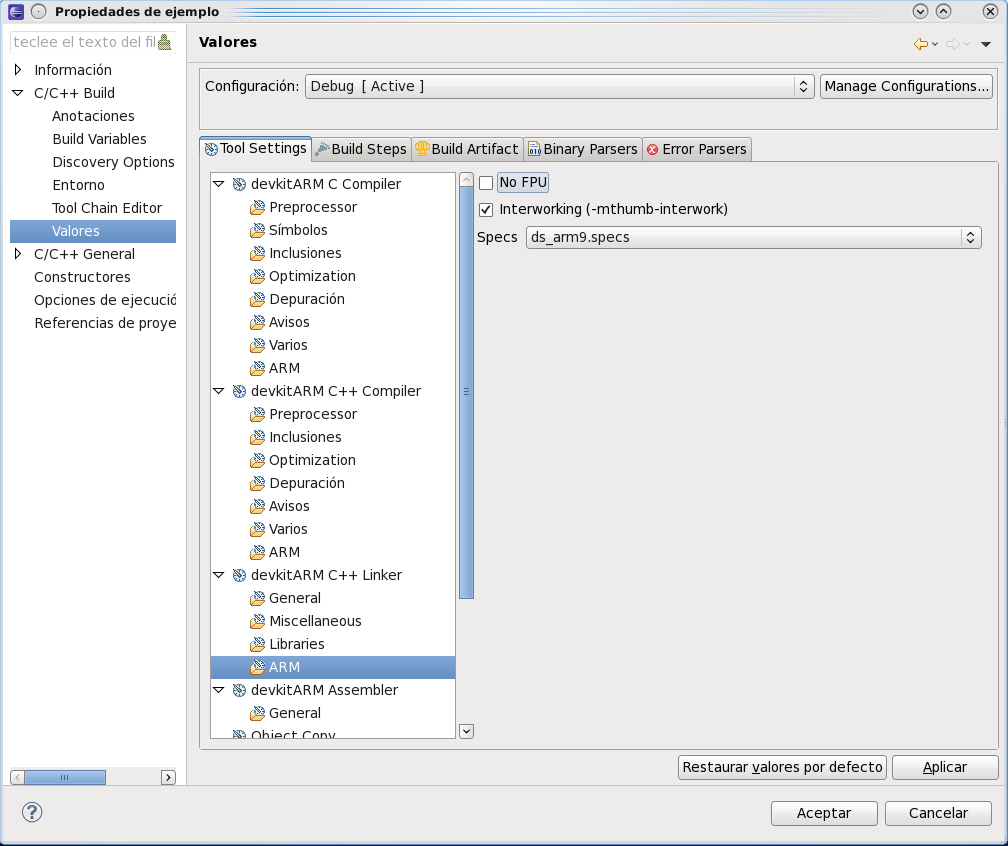
\includegraphics[height=7cm]{./Figuras/C2/c2_instan8.png}
	\caption{Creación de un proyecto para NDS usando Eclipse en Linux (parte 8).}
	\label{fig_pig_p3_c1_eclipel8}
\end{figure}


% --------------------------------------------------------------------------
\subsubsection{Edición del fichero ejemplo}
Para familiarizarse con el entorno de desarrollo de \textit{Eclipse} para NDS, se utiliza el mismo ejemplo que el del apartado anterior.  En primer lugar, se debe crear un fichero fuente en \textit{lenguaje C} dentro del proyecto actual. Para ello se pulsa en \textit{Archivo->Nuevo->Source File}. Aparece una nueva ventana (\textit{New Source File}) (ver Figura \ref{fig_pig_p3_c1_eclipel9}).

\begin{figure}[t]
	\centering
	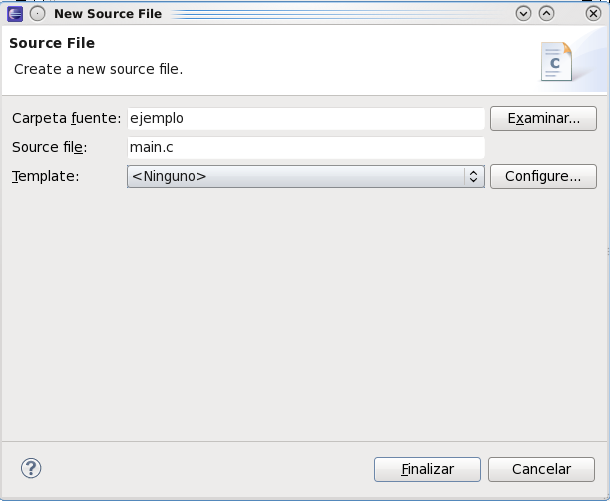
\includegraphics[height=7cm]{./Figuras/C2/c2_instan9.png}
	\caption{Creación de un proyecto para NDS usando Eclipse en Linux (parte 9).}
	\label{fig_pig_p3_c1_eclipel9}
\end{figure}


\noindent en la que se debe realizar lo siguiente:
\begin{itemize}
 	\item En \textit{Source File} se introduce \textit{main.c}.
 	\item En \textit{Template} se selecciona \textit{Ninguno}.
 	\item Se pulsa en \textit{Finalizar}.
\end{itemize}

A continuación en la ventana que hace referencia a \textit{main.c} se introduce el mismo código que el del apartado \ref{sec:programa}.

% --------------------------------------------------------------------------
\subsubsection{Compilación del fichero ejemplo}
El siguiente paso es compilar el programa, para ello se elige \textit{Proyecto->Construir proyecto}. Si no se han producido errores de compilación aparecerá el fichero \textit{ejemplo.nds} en el directorio \textit{Debug}. Si se produjese un error relacionado con que no encuentra el compilador se puede realizar lo siguiente:

\begin{itemize}
\item Hacer una copia de los siguientes ficheros que se encuentran en \textit{/opt/devkitpro/devkitARM/bin}:	
 \begin{itemize}
 	\item arm-none-eabi-as
 	\item arm-none-eabi-g++
 	\item arm-none-eabi-gcc	
 	\item arm-none-eabi-gdb
   \item arm-none-eabi-objcopy
 \end{itemize}
 	\item Renombrar las copias con los siguientes nombres:	
 \begin{itemize}
 	\item arm-eabi-as
 	\item arm-eabi-g++
 	\item arm-eabi-gcc	
 	\item arm-eabi-gdb
   \item arm-eabi-objcopy
 \end{itemize}
\end{itemize}

% --------------------------------------------------------------------------
\subsubsection{Ejecución del fichero ejemplo en el emulador}
Una vez abierto \textit{WinDS Pro}, si se escoge el emulador \textit{No\$gba}, se pulsa en \textit{File->Cartridge Menu (File Name)} y se busca el fichero \textit{.nds} que nos interesa. Si se escoge el emulador \textit{DeSmuME}, se pulsa en \textit{File->Open ROM} y se busca el fichero \textit{.nds} que nos interesa.

 % Herramientas para programar la NDS
\chapterimage{chapter_head_1.pdf} 
\chapter{Fundamentos para programar la NDS}

En este capítulo, se estudiarán los elementos básicos para poder realizar aplicaciones en la consola NDS. En concreto, se estudiarán cuestiones relacionadas con la visualización de texto, la entrada de usuario (botones y pantalla táctil) y el temporizador. 

Para obtener información sobre las funciones existentes, se recomienda ir a la página web: \url{http://libnds.devkitpro.org/}

La lista de ejercicios a realizar y el tiempo estimado (en minutos) para su realización se muestran en la Tabla \ref{c3_tab:ejercios}.

\begin{table}[t]
\centering
\caption{Ejercicios del capítulo y tiempo estimado para su realización.}
\begin{tabular}{|c|c|c|c|}
\hline 
Ejercicio & Tiempo & Ejercicio & Tiempo  \\ 
\hline 
 3.1 & 30' & 3.10 & 10' \\ 
 3.2 & 10' & 3.11 & 20' \\ 
 3.3 & 5'  & 3.12 & 20' \\ 
 3.4 & 5'  & 3.13 & 10' \\ 
 3.5 & 10' & 3.14 & 30' \\ 
 3.6 & 10' & 3.15 & 10' \\ 
 3.7 & 20' & 3.16 & 10' \\ 
 3.8 & 15' & 3.17 & 10' \\ 
 3.9 & 15' &      & \\ 
\hline 
\end{tabular} 
\label{c3_tab:ejercios}
\end{table}
% ---------------------------------------------------------
% ---------------------------------------------------------
\section{Introducción a la programación en NDS}
La estructura básica de las aplicaciones realizadas para NDS es la siguiente:

\begin{lstlisting}
#include [...] 
int main(void)
{
	inicializar libNDS; 
	while(1){
		// Bucle principal 
	}
	return 0;
}
\end{lstlisting}

El bucle infinito sirve para simular el comportamiento de un videojuego al entrar en su bucle principal. El formato habitual de estos tipos de bucles es el siguiente:

\begin{verbatim}
Comienza el bucle:
    Comprobar la entrada de usuario
    Actualizar la lógica interna
    Comprobar el criterio de finalización del bucle
    Redibujar
Fin del bucle
\end{verbatim}



\begin{example}
	El siguiente código muestra un mensaje de texto por la pantalla:
\begin{lstlisting}
#include<nds.h>
#include<stdio.h>
int main(void) {
  consoleDemoInit();
  iprintf("Me gusta programar videojuegos");  // Imprimir el mensaje 
  while(1) 
  {} // Bucle que no hace nada.     
}
\end{lstlisting}
\end{example}


\begin{exercise}
	Crea un nuevo proyecto usando el código anterior para comprobar que tienes bien instalado todo lo necesario para compilar y ejecutar juegos en la NDS. El capítulo 2 está dedicado a explicar todos los pasos que hay que seguir. 
\end{exercise}

 ---------------------------------------------------------
% ---------------------------------------------------------
\section{Salida de texto}
La Nintendo DS tiene dos pantallas gráficas de tipo LCD (\textit{Liquid Crystal Display}). Las dos tienen el mismo tamaño, 256x192 píxeles, y funcionan gracias a dos motores gráficos: principal o \textit{main} y secundario o \textit{sub}. Además, la pantalla inferior emplea tecnología táctil.

% ---------------------------------------------------------
% ---------------------------------------------------------
\subsection{Visualización de texto en la pantalla}
La pantalla tiene 32 columnas y 24 filas para visualizar texto, tal y como se puede observar en la Figura \ref{fig_c3_texto}. La instrucción \textit{iprintf} se emplea para visualizar texto por la pantalla. Para elegir la posición del texto en la pantalla se usa la secuencia de escape:
\begin{verbatim}
\x1b[<fila>;<columna>H
\end{verbatim}
empleando como valor para la fila un entero entre 0 y 23, y el valor de la columna, un entero entre 0 y 31.

\begin{figure}[t]
\centering
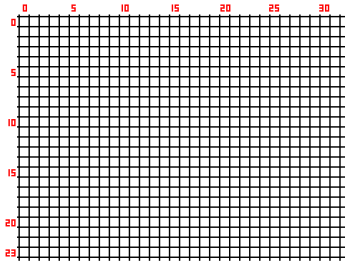
\includegraphics[height=6cm]{Figuras/C3/c3_eclipse12.png}
\caption{Pantalla de la NDS}
\label{fig_c3_texto}
\end{figure}

\begin{example}
El siguiente código muestra un mensaje de texto en la fila 2, columna 5:
\begin{lstlisting}
#include <nds.h>
#include <stdio.h>
int main(void)
{
  consoleDemoInit(); 
  int fila    = 2;
  int columna = 5;
  while(1) {
  	iprintf("\x1b[%d;%dHMensaje de texto", fila, columna);
  	swiWaitForVBlank();  
  }
  return 0;
}
\end{lstlisting}
\end{example}

\begin{exercise}
Realiza un programa que muestre un mensaje de texto aproximadamente en el centro de la pantalla. 
\end{exercise}

\begin{exercise}
Realiza un programa que muestre tres mensajes de texto en varias posiciones diferentes de la pantalla. 
\end{exercise}

% ---------------------------------------------------------
% ---------------------------------------------------------
\subsection{Control de las pantallas a utilizar}
\begin{example}
El siguiente programa (\textit{superior.c}) crea una consola para escribir en la pantalla superior:
\begin{lstlisting}
#include <nds.h>
#include <stdio.h>
int main(void)
{
  PrintConsole pantalla;

  videoSetMode(MODE_0_2D);

  consoleInit(
  		&pantalla,        // Consola a inicializar
	    3,                // Capa del fondo donde se imprimirá
	    BgType_Text4bpp,  // Tipo de fondo
	    BgSize_T_256x256, // Tamaño del fondo
	    31,               // Base del mapa
	    0,                // Base del tile gráfico
	    true,             // Sistema grafico a usar (main system)
	    true);            // No cargar gráficos para la fuente

  while(1) {
  iprintf("\x1b[12;10HMensaje de texto");
  swiWaitForVBlank();    // Esperar al refresco de pantalla
  }
  return 0;
}
\end{lstlisting}
\end{example}

En este código cabe destacar lo siguiente:
\begin{itemize}
\item \textit{PrintConsole} es el tipo de datos que define las consolas a utilizar a la hora de imprimir contenidos en pantalla. Se declara la variable \textit{pantalla} de este tipo.
%    
\item La función \textit{VideoSetMode} se encarga de inicializar el sistema gráfico principal (\textit{main}), que es el que se usa en el ejemplo. Si se quiere imprimir en la pantalla inferior, se debería inicializar con \textit{VideoSetModeSub}. Los modos de vídeo soportados (en este caso \textit{MODE\_0\_2D})  dependen del sistema y el fondo que se estén utilizando, y se verán con más detalle en próximos capítulos.
%
\item Para crear una consola con los parámetros deseados se usará la función \textit{consoleInit}. Esta función tiene ocho parámetros de entrada, de los cuales el único que por ahora interesa es el penúltimo que indica el sistema gráfico que se va a usar: con el valor \textit{true}, se utilizará el sistema principal (la pantalla superior), mientras que con el valor \textit{false}, se imprimirá en la pantalla inferior.  \item La función \textit{swiWaitForVBlank} espera al refresco de la pantalla.
\end{itemize}

\begin{exercise}
Crea un nuevo proyecto, usando el programa \textit{superior.c} y comprueba que el resultado obtenido es el esperado.
\end{exercise}

Para usar más de una consola, se deben seguir los pasos del ejemplo anterior, pero además se debe emplear la función \textit{consoleSelect} para indicar qué consola se va a usar. 

\begin{example}
El siguiente programa (\textit{dos\_pantallas.c}) escribe un mensaje en cada una de las pantallas:

\begin{lstlisting}
#include <nds.h>
#include <stdio.h>
int main(void)
{
  PrintConsole pantalla_sup, pantalla_inf;  
  videoSetMode   (MODE_0_2D);
  videoSetModeSub(MODE_0_2D);
  
  consoleInit(&pantalla_sup, 
              3, 
              BgType_Text4bpp,
              BgSize_T_256x256, 
              31, 
              0,
              true, 
              true);
  consoleInit(&pantalla_inf,
              3,
              BgType_Text4bpp,
              BgSize_T_256x256,
              31,
              0,
              false,
              true);

  while(1) {  
   consoleSelect(&pantalla_sup);
   iprintf("\x1b[12;3HEsta es la pantalla superior.");
   consoleSelect(&pantalla_inf);
   iprintf("\x1b[12;3HEsta es la pantalla inferior.");

   swiWaitForVBlank();
  }
  return 0;
}
\end{lstlisting}
\end{example}

\begin{exercise}
Comprueba mediante la creación de un nuevo proyecto, usando el programa \textit{dos\_pantallas.c} que lo indicado ocurre tal y como se comenta. La Figura \ref{p3_c2_dos_pantallas} muestra la salida esperada.
\end{exercise}


\begin{exercise}
	Realiza un programa que muestre tres mensajes en la pantalla superior y otros tres en la pantalla inferior.
\end{exercise}

\begin{figure}[t]
\centering
 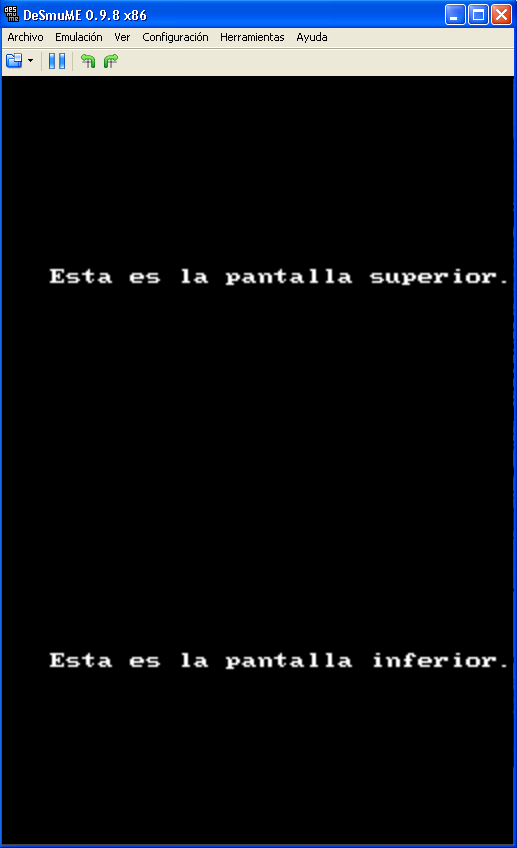
\includegraphics[height=9cm]{Figuras/C3/c3_sol-ejercicios-dospantallas.png}
\caption{Resultado del programa \textit{dos\_pantallas.c}.}
\label{p3_c2_dos_pantallas}
\end{figure}

% ---------------------------------------------------------
% ---------------------------------------------------------
\section{Teclado}
La Nintendo DS tiene la posibilidad de simular el funcionamiento de un teclado empleando funciones de la biblioteca \textit{libnds}.

\begin{example}
El siguiente programa (\textit{teclado.c}) muestra como funciona el acceso al teclado:

\begin{lstlisting}
#include <nds.h>
#include <stdio.h>
int main(void) {    
  int key;  // Variable que almacena el código ascii de la tecla
    
  consoleDemoInit();  
  keyboardDemoInit();  // Inicializa un teclado
  keyboardShow();      // Visualiza el teclado

  while(1) {       
    key = keyboardUpdate();  // Procesa la tecla pulsada
                             // Retorna el código ascii 
                             // -1 si no se ha pulsado tecla 

    // Visualiza el carácter asociado al ascii de la tecla 
    if (key > 0) iprintf("Tecla pulsada %c \n", key); 

    swiWaitForVBlank(); 
  }
  return 0;
}
\end{lstlisting}
\end{example}

Este programa visualiza la tecla pulsada, para ello se ha introducido el formato \textit{\%c} en la instrucción \textit{iprintf} para visualizar un carácter. La salida del programa \textit{teclado.c} en el emulador se muestra en la Figura \ref{fig_c3_teclado1}.

\begin{figure}[t]
\centering
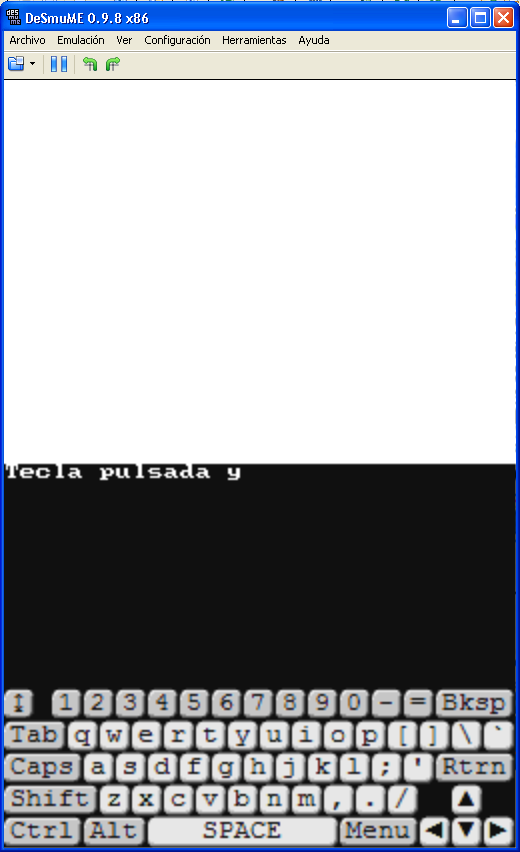
\includegraphics[height=8cm]{Figuras/C3/c3_teclado1.png}
\caption{Salida del programa \textit{teclado.c} en el emulador.}
\label{fig_c3_teclado1}
\end{figure}

En la página web \url{http://libnds.devkitpro.org/keyboard_8h.html} se encuentra más información sobre el funcionamiento del teclado de la NDS.


\begin{exercise}
A partir del código del programa \textit{teclado.c}, crea un programa que muestre tu nombre cuando se pulse y se mantenga pulsada una tecla cualquiera y que deje de mostrarlo cuando se deje de pulsar la tecla.
\end{exercise}

\begin{exercise}
A partir del código del programa \textit{teclado.c}, crea un programa que de inicio muestre tu nombre, pero cuando se pulse una tecla cualquiera deje de mostrarlo. Si de nuevo se pulsa una tecla se volverá a mostrar, y así sucesivamente.
\end{exercise}

\begin{exercise}
A partir del código del programa \textit{teclado.c}, crea un programa que muestre tu nombre cuando se pulse la tecla \textit{s}. El nombre continuará visible hasta que se pulse la tecla \textit{n}. Si se vuelve a pulsar la tecla \textit{s}, el nombre volverá a ser visible y así sucesivamente.
\end{exercise}

% ---------------------------------------------------------
% ---------------------------------------------------------
\section{Botones de la consola}
La consola NDS presenta los siguientes botones como entrada de usuario (ver Figura \ref{fig_c3_botones}):
\begin{itemize}
\item Una cruceta direccional a la izquierda de la pantalla inferior (cruceta de 4 direcciones).
%
\item Cuatro botones (\textit{A}, \textit{B}, \textit{X}, \textit{Y}) a la derecha de la pantalla inferior.
%
\item Dos botones laterales (\textit{L} y \textit{R}) situados detrás.
%
\item Botón de \textit{Select} y botón de \textit{Start}, a la derecha de la pantalla inferior.
%
\item La pantalla táctil inferior.
\end{itemize}

\begin{figure}[t]
\centering
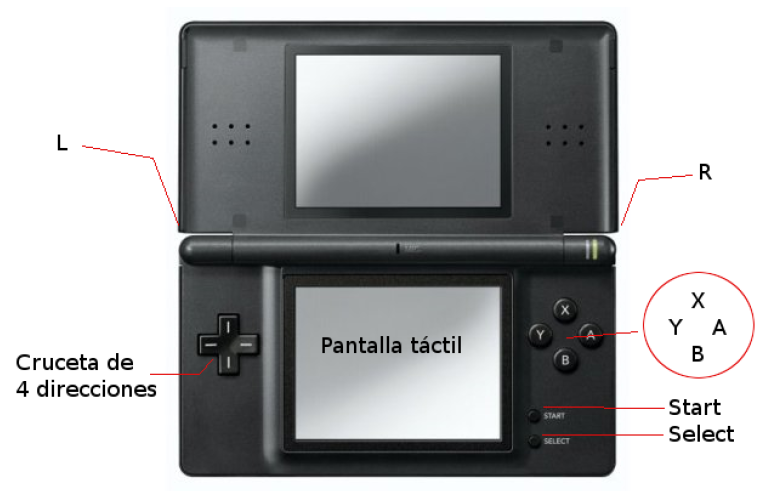
\includegraphics[height=7cm]{Figuras/C3/c3_botones.png}
\caption{Botones de la NDS.}
\label{fig_c3_botones}
\end{figure}

Además, el cierre de la consola tiene también un sensor para saber si está abierta o cerrada, que a efectos de programación, funciona como otro botón más.

La Figura \ref{fig_c3_botones_teclass} muestra la relación que existe entre los botones de la NDS y el teclado en un determinado emulador.

\begin{figure}[t]
\centering
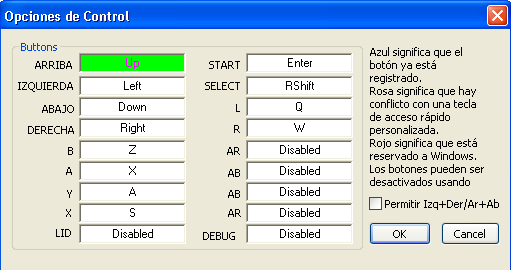
\includegraphics[height=5.5cm]{Figuras/C3/c3_botones_teclas.png}
\caption{Relación que existe entre los botones de la NDS y el teclado.}
\label{fig_c3_botones_teclass}
\end{figure}

Los pasos a seguir para determinar las operaciones realizadas con los botones son los siguientes:
\begin{enumerate}
\item Primero, en cada paso por el bucle principal, se determinará si se ha pulsado algunos de los botones mediante la función \textit{scanKeys}. 
%
\item Después se puede  obtener información sobre los botones con las siguientes funciones:
\begin{itemize}
	\item \textit{keysCurrent}: obtiene el estado actual de los botones.
	\item \textit{keysDown}: obtiene los botones pulsados en ese instante.
	\item \textit{keysHeld}: obtiene los botones mantenidos.
	\item \textit{keysUp}: obtiene los botones liberados.
\end{itemize}
\end{enumerate}

El resultado de estas funciones se compara mediante una \textit{multiplicación bit a bit} con el valor del botón del que se quiere saber su estado. Como valores del botón cuyo estado se desea saber se puede emplear: 
\begin{itemize}
\item Los cuatro botones de la derecha: KEY\_A, KEY\_B, KEY\_X, KEY\_Y.
\item Los botones laterales \textit{L} y \textit{R}: KEY\_L, KEY\_R.
\item Botones \textit{Select} y \textit{Start}: KEY\_SELECT, KEY\_START.
\item La cruceta de 4 direcciones: KEY\_UP, KEY\_DOWN, KEY\_LEFT, KEY\_RIGHT.
\item La pantalla táctil (solo como botón): KEY\_TOUCH.
\item La bisagra del cierre de la consola: KEY\_LID.
\end{itemize}

La siguiente página web contiene información sobre el uso de la botonera \url{http://libnds.devkitpro.org/arm9_2input_8h.html}

\begin{example}
El siguiente programa (\textit{botones.c}) comprueba el estado instantáneo de cada botón, mostrando en pantalla si se ha pulsado: 
\begin{lstlisting}
#include <nds.h>
#include <stdio.h>
int main()
{
  u32 keys;
  consoleDemoInit();

  while(1){
    scanKeys();
    keys = keysCurrent(); // Se lee el estado actual de todos los botones

    // Se comprueba si se ha pulsado arriba en la cruceta
    if (keys & KEY_UP) iprintf("\x1b[10;5H Pulsado UP");
    else               iprintf("\x1b[10;5H           ");

   // Se comprueba si se ha pulsado en el boton A
   if (keys & KEY_A)   iprintf("\x1b[12;5H Pulsado A");
   else                iprintf("\x1b[12;5H          ");

   // Se comprueba si se ha pulsado el botón Start
   if (keys & KEY_START) iprintf("\x1b[15;5H Pulsado START");
   else                  iprintf("\x1b[15;5H              ");

   // Se comprueba si se ha pulsado la pantalla táctil
   if (keys & KEY_TOUCH) iprintf("\x1b[13;5H Pantalla tactil");
   else                  iprintf("\x1b[13;5H                ");

   swiWaitForVBlank();
  }
  return 0;
}
\end{lstlisting}
\end{example}
	
Se puede observar que se llama a la función \textit{scanKeys}, y que posteriormente se llama a la función \textit{keysCurrent} para conocer el estado actual de los botones. Dicha información se guarda en la variable \textit{keys}, declarada de tipo \textit{u32} (entero sin signo de 32 bits). Con el valor de esta variable se realiza la multiplicación bit a bit con el valor de un botón específico mediante:
\begin{lstlisting}
if (keys & KEY_UP)
\end{lstlisting}

Si el botón está pulsado, se muestra en pantalla un mensaje indicando el  botón en concreto, incluyendo la pantalla táctil. Si se quieren realizar
acciones en momentos precisos (justo cuando se pulsa un botón, o cuando se libera), se podrán utilizar el resto de funciones.

\begin{exercise}
Comprueba mediante la creación de un nuevo proyecto, usando el código \textit{botones.c}, que lo indicado ocurre tal y como se comenta.
\end{exercise}

\begin{exercise}
Realiza un programa que permita desplazar un mensaje de texto por la pantalla inferior empleando los botones de dirección (derecha, izquierda, arriba y abajo). Se debe controlar que el mensaje completo siempre se encuentre dentro de la pantalla, y que se desplace solo una posición en cada pulsación del correspondiente botón.
\end{exercise}

\begin{exercise}
Modifica el programa anterior para que al pulsar el botón \textit{X} se cambie el mensaje a mostrar por otro mensaje. Al pulsar el botón \textit{B} se deberá volver a mostrar el mensaje original.
\end{exercise}

% ---------------------------------------------------------
% ---------------------------------------------------------
\section{Pantalla táctil}
\label{sec_pantalla_tactil}
Como ya se ha comentado, la pantalla inferior emplea tecnología táctil. En la Nintendo DS se usa el  sistema de coordenadas cartesiano mostrado en la Figura \ref{fig_c3_cartesiano}. En el emulador se emplea el ratón como puntero de la pantalla táctil.

La siguiente página web contiene información sobre el uso de la pantalla táctil  \url{http://libnds.devkitpro.org/arm9_2input_8h.html}

\begin{example}
El siguiente programa (\textit{tactil.c}) cuenta el número de veces que se pulsa en la pantalla táctil.

\begin{figure}[t]
\centering
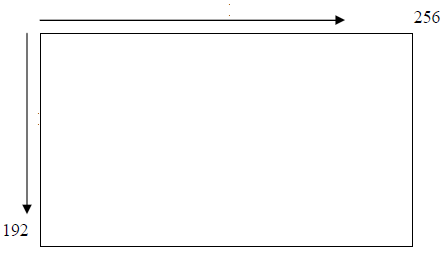
\includegraphics[height=7cm]{Figuras/C3/c3_coordenadas.png}
\caption{Sistema de coordenadas cartesiano usado para detectar donde ha pulsado el usuario en la pantalla táctil.}
\label{fig_c3_cartesiano}
\end{figure}

\begin{lstlisting}
#include <nds.h>
#include <stdio.h>

int main(void) {
  touchPosition posicionXY;
  int           contador;

  consoleDemoInit();
  contador = 0;

  while(1)
  {
    scanKeys();
    touchRead(&posicionXY); // Se lee la posición actual.
    iprintf("\x1b[1;0HPosicion x=%04i y=%04i ",
            posicionXY.px, 
            posicionXY.py);
    iprintf("\x1b[2;0HContador=%04i", 
            contador);

    if (keysDown() & KEY_TOUCH) contador++;

    swiWaitForVBlank();
  }
  return 0;
}
\end{lstlisting}
\end{example}

De este código se puede destacar lo siguiente:
\begin{itemize}
\item Se crea una variable del tipo \textit{touchPosition} (en este caso \textit{posicionXY}) para reconocer la posición del puntero en la pantalla táctil. Mediante \textit{posicionXY.px} se obtiene la posición respecto al eje \textit{x}, mientras que con \textit{posicionXY.py} se obtiene la posición respecto al eje \textit{y}.
%
\item La función \textit{touchRead} lee el valor de la posición del puntero en la pantalla táctil.
%
\item El formato \textit{\%04i} en la instrucción \textit{iprintf}  visualiza un número entero de 4 cifras (en decimal)  poniendo ceros en la izquierda. 
\end{itemize}

\begin{exercise}
	Comprueba mediante la creación de un nuevo proyecto, usando el código \textit{tactil.c}, que lo indicado ocurre tal y como se comenta.
\end{exercise}

\begin{exercise}
Realiza un programa que divida la pantalla inferior en 4 zonas. En cada una de ellas deberá aparecer un contador que contará el número de veces que se pulsa en cada zona. La Figura \ref{fig_p3_c3_4zonas} muestra un ejemplo de la salida del programa requerido.
\end{exercise}

\begin{figure}[t]
\centering
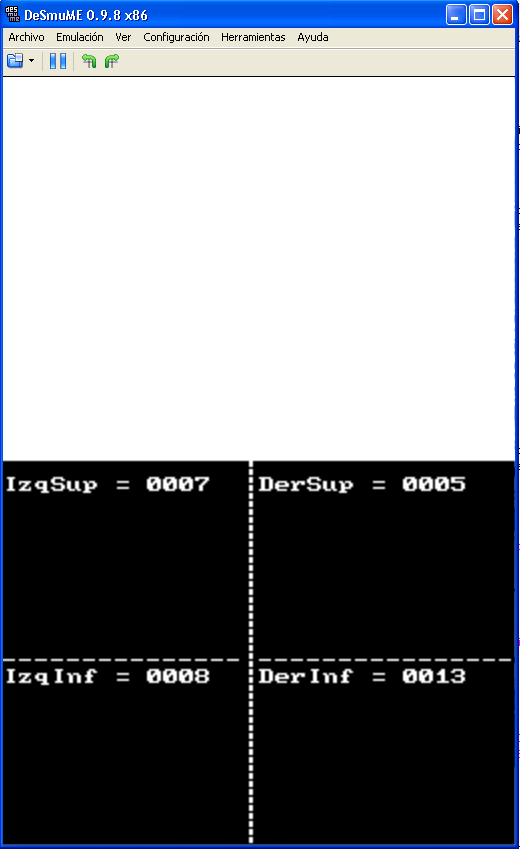
\includegraphics[height=7.5cm]{Figuras/C3/c3_tactil1.png}
\caption{Salida ejemplo del programa requerido en la sección \ref{sec_pantalla_tactil}}
\label{fig_p3_c3_4zonas}
\end{figure}

% ---------------------------------------------------------
% ---------------------------------------------------------
\section{Temporizador}
La Nintendo DS cuenta con temporizadores (\textit{timers}) de tiempo real, que pueden ser empleados por una aplicación o juego para definir diferentes respuestas dependiendo de la hora del día. Las características que tienen son las siguientes:

\begin{itemize}
	\item Hay 8 temporizadores de 16 bits, 4 en el ARM9 y 4 en el ARM7.
	\item Funcionan como contadores de eventos.
	\item La frecuencia base con la que trabajan es de 33MHz, sobre la que se puede aplicar los siguientes divisores de frecuencia: 1, 64, 256 y 1024.
	\item Soportan la configuración en cascada, es decir, que cuando un temporizador se desborda el si\-guien\-te temporizador incrementa su cuenta.
	\item Pueden generar interrupciones. 
\end{itemize}

La página web \url{http://libnds.devkitpro.org/timers_8h.html} muestra información sobre los temporizadores.

\begin{example}
El siguiente programa (\textit{tiempo.c}) muestra el tiempo que va transcurriendo en segundos:
\begin{lstlisting}
#include <nds.h>
#include <stdio.h>
#include <time.h>
//se define la velocidad del reloj con ClockDivider_1024
#define TIMER_SPEED (BUS_CLOCK/1024)
int main()
{
  consoleDemoInit();
  uint ticks = 0;
  timerStart(0, ClockDivider_1024, 0, NULL); // Iniciar el reloj
  while (1)
  {
   ticks += timerElapsed(0);  
   iprintf("\x1b[1;0Hticks:  %u",ticks);
   iprintf("\x1b[2;0Hseg.: %u:%u",
           ticks/TIMER_SPEED,
           ((ticks%TIMER_SPEED)*1000)/TIMER_SPEED);
   swiWaitForVBlank();
  }
  return 0;
}
\end{lstlisting}
\end{example}
	
Se declara la variable \textit{ticks} como \textit{uint} (entero sin signo). En la llamada \textit{timerStart} cabe destacar lo si\-guien\-te:
\begin{itemize}
\item El primer parámetro hace referencia al \textit{temporizador 0}.
%
\item El parámetro \textit{ClockDivider\_1024} hace referencia a aplicar una división de frecuencia de 1024.
\end{itemize}

La función \textit{timerElapsed} proporciona el número de ticks que se han producido desde la última llamada a esa misma función, para el temporizador especificado (en este caso el 0).  El formato \textit{\%u} en la instrucción \textit{iprintf}  visualiza un número entero sin signo.

\begin{exercise}
	Comprueba mediante la creación de un nuevo proyecto, usando el código \textit{tiempo.c}, que lo indicado ocurre tal y como se comenta.
\end{exercise}

\begin{exercise}
Modifica el programa \textit{tiempo.c} para que finalice la cuenta si han transcurrido 15 segundos o si se ha pulsado el boton \textit{Y}.
\end{exercise}

En ocasiones se desea que ocurra un evento cada cierto tiempo. 

\begin{example}
El siguiente programa (\textit{eventos.c}) mueve la letra \textit{X} hacia la derecha cada 2 segundos:

\begin{lstlisting}
#include <nds.h>
#include <stdio.h>
#include <time.h>

#define TIMER_SPEED (BUS_CLOCK/1024)

int main()
{
  consoleDemoInit();
  uint ticks          = 0;
  int  posicion       = 0;
  int  proximo_cambio = 2;
  int  segundos;
  
  timerStart(0, ClockDivider_1024, 0, NULL);

  while (1)
  {
    ticks   += timerElapsed(0);
    segundos = (int) (ticks/TIMER_SPEED);

    if (segundos >= proximo_cambio)
    {
      posicion       = posicion       + 1;
      proximo_cambio = proximo_cambio + 2;
    }
    iprintf("\x1b[1;%dH ", posicion-1); // Borra anterior
    iprintf("\x1b[1;%dHX", posicion);   // Dibuja X
    swiWaitForVBlank();
  }
  return 0;
}
\end{lstlisting}
\end{example}
	
\begin{exercise}
	Modifica el programa \textit{eventos.c} para que la letra se mueva cada 3 segundos.
\end{exercise}

Es importante destacar que para programar este tipo de funcionalidad, es más conveniente el uso de interrupciones, tal como se verá posteriormente.

 % Fundamentos para programar la NDS
%\chapterimage{chapter_head_1.pdf} 
\chapter{Programación de un juego sin gráficos}

En este capítulo, se darán las instrucciones para la realización paso a paso un videojuego sin usar el sistema gráfico de la NDS.

La lista de ejercicios y el tiempo estimado (en minutos) para su realización se muestran en la Tabla \ref{c4_tab:ejercios}.

\begin{table}[t]
\centering
\caption{Ejercicios del capítulo y tiempo estimado para su realización.}
\begin{tabular}{|c|c|}
\hline 
Ejercicio & Tiempo \\ 
\hline 
 4.1 & 10' \\ 
 4.2 & 20' \\ 
 4.3 & 30' \\ 
 4.4 & 20' \\ 
 4.5 & 10' \\ 
 4.6 & 10' \\ 
 4.7 & 10' \\ 
 4.8 & 10' \\ 
\hline 
\end{tabular} 
\label{c4_tab:ejercios}
\end{table}

% ---------------------------------------------------------
% ---------------------------------------------------------
\section{Descripción del juego}
El juego que se va a realizar es una versión simplificada del típico juego de carreras de caballos que se solían encontrar en las ferias itinerantes. La Figura \ref{fig_c4_caballos}\footnote{La imagen se ha obtenido en la siguiente web: \url{http://www.parquedebolas.com/images/productos/gran/523000002.jpg}} muestra un ejemplo de este tipo de juego. En este juego, el usuario debe introducir bolas en unos agujeros, y según el agujero donde ha caído la bola, el caballo irá más o menos deprisa. Gana el caballo que antes llegue a la meta.

\begin{figure}[t]
	\centering
	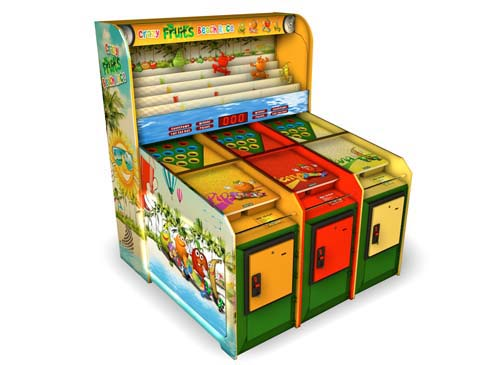
\includegraphics[height=7cm]{Figuras/C4/c4_caballos.jpg}
	\caption{Juego de las carreras de caballos.}
	\label{fig_c4_caballos}
\end{figure}

En la versión que se va a desarrollar se usarán los conceptos aprendidos en el capítulo 3. En la pantalla superior se mostrará la carrera. La pantalla se dividirá en 4 carriles horizontales, uno por caballo. Para representar cada caballo se usará una letra. Al inicio los 4 caballos se situarán en la primera columna de la pantalla (columna 0). Ganará el primer caballo que alcance la meta situada en la última columna de la pantalla (columna 31).

En la pantalla inferior habrá un mensaje indicando el dinero que tiene el jugador. Al inicio el jugador tendrá 1000 euros.

También existirán cuatro botones, uno por caballo. El jugador deberá pulsar en uno de los cuatro botones para apostar por un caballo determinado. La apuesta es de 100 euros. Si el caballo por el que ha apostado el jugador gana, se obtendrán 200 euros que serán añadidos al dinero total. Si gana otro caballo, el jugador perderá ese dinero.

El juego continuará hasta que el jugador se quede sin dinero o alcance la cifra de 10 000 euros.

\section{Desarrollo del juego}

\begin{example}
El siguiente listado (\textit{caballos\_inicial.c}) muestra el esqueleto del programa que puedes usar para empezar:
\begin{lstlisting}
#include <nds.h>
#include <stdio.h>

void MostrarCaballos(int posicion_caballos[]);
void MostrarBotones();
void MostrarDinero(int dinero);

int main(void)
{
  PrintConsole pantalla_sup, pantalla_inf;
  videoSetMode   (MODE_0_2D);
  videoSetModeSub(MODE_0_2D);
  consoleInit (&pantalla_sup, 3, BgType_Text4bpp, 
               BgSize_T_256x256, 31, 0, true, true);
  consoleInit (&pantalla_inf, 3, BgType_Text4bpp, 
               BgSize_T_256x256, 31, 0, false, true);

  int posicion_caballos[4];
  for (int i=0; i<4; i++)
    posicion_caballos[i] = 0;
    
  int dinero = 1000;   

  while(1)
  {
    consoleSelect  (&pantalla_sup);
    MostrarCaballos(posicion_caballos);
    consoleSelect  (&pantalla_inf);
    MostrarDinero  (dinero);
    MostrarBotones ();
  }
}

void MostrarCaballos(int posicion_caballos[])
{
  iprintf("\x1b[2;%dHA", posicion_caballos[0]);
  iprintf("\x1b[8;%dHB", posicion_caballos[1]);
  iprintf("\x1b[14;%dHC",posicion_caballos[2]);
  iprintf("\x1b[20;%dHD",posicion_caballos[3]);
}

void MostrarBotones()
{
  iprintf("\x1b[10;1HApuesta por un caballo: ");
  iprintf("\x1b[12;4H----- ----- ----- -----");
  iprintf("\x1b[13;4H- A - - B - - C - - D -");
  iprintf("\x1b[14;4H----- ----- ----- -----");
}

void MostrarDinero(int dinero)
{
  iprintf("\x1b[2;1HTienes %d euros", dinero);
}
\end{lstlisting}
\end{example}
	
Como se puede comprobar por el código anterior, los cuatro carriles para mostrar la evolución de los caballos estarán en las filas, 2, 8, 14 y 20 de la pantalla superior. En la fila 2 de la pantalla inferior se mostrará un mensaje indicando el dinero que tiene el jugador. En las filas 12, 13 y 14 se mostrarán los botones para apostar por los caballos.

\begin{exercise}
	Crea un nuevo proyecto usando el código \textit{caballos\_inicial.c} y comprueba que funciona correctamente.
\end{exercise}

Para crear el programa completo debes resolver los siguientes ejercicios en el orden establecido. En primer lugar debes crear el código necesario para que los caballos se muevan hacia la meta. Al inicio todos los caballos tendrán una velocidad de una posición por unidad de tiempo. Antes de mostrar la posición de los caballos (función \textit{MostrarCaballos}), debes llamar a una función de nombre \textit{ActualizarPosicionCaballos} que dada la posición actual y la velocidad actual de cada caballo, actualice su posición. Debes tener en cuenta que la máxima posición que puede tener un caballo es la columna 31 y la mínima la 0. Así mismo, la mínima velocidad de un caballo es 0, y la máxima un valor que establezcas (por ejemplo 3).

Cada vez que actualices la posición de los caballos debes borrar la pantalla superior, para ello debes crear una funcion \textit{BorrarPantalla} que será llamada antes de mostrar los caballos en la nueva posición.

Por último debes crear una función \textit{ComprobarGanador} que devolverá el número de caballo que ha llegado a la meta o -1 si no ha llegado todavía ninguno. En caso de empate, el ganador será siempre el que tenga el número menor. Por ejemplo, si llegan a la vez el 0 (letra A) y el 1 (letra B), el ganador será el 0.

\begin{example}
El programa principal, con los cambios comentados, es el siguiente:

\begin{lstlisting}
...
  int velocidad_caballos[4];
  for (int i=0; i<4; i++)
    velocidad_caballos[i] = 1;
...
  int hay_ganador = 0;
  while(1)
  {
    if (hay_ganador == 0)
    {
      int ganador = ComprobarGanador(posicion_caballos);
      if (ganador >= 0)
      {
        hay_ganador = 1;
        consoleSelect(&pantalla_inf);
        iprintf("\x1b[5;1HEl caballo ganador es el: %d",ganador);
      }
      else
      {
        ActualizarPosicionCaballos(posicion_caballos, velocidad_caballos);      
        consoleSelect(&pantalla_sup);
        BorrarPantalla();
        MostrarCaballos(posicion_caballos);
      }
    }
    consoleSelect(&pantalla_inf);
    MostrarDinero(dinero);
    MostrarBotones();
}
...
\end{lstlisting}
\end{example}

Como puedes comprobar en el código anterior, la fila 5 de la pantalla inferior se usará para mostrar el caballo ganador.

\begin{exercise}
	Implementa las funciones \textit{BorrarPantalla}, \textit{ActualizarPosicionCaballos} y \textit{ComprobarGanador}.
\end{exercise}

Si el código funciona correctamente, habrás comprobado que los 4 caballos llegan a la vez a la meta, puesto que su velocidad es siempre la misma. Por lo tanto, el ganador es siempre el caballo 0. Además, puesto que en cada frame se actualiza la posición, el movimiento de los caballos no se aprecia. 

Para solucionar el primer problema, debes modificar la función \textit{ActualizarPosicionCaballos} para que dependiendo de un número aleatorio, la velocidad de los caballos pueda variar. Para modificar la velocidad de los caballos, se puede usar un generador de números aleatorios entre dos números reales usando la siguiente función \footnote{Código obtenido de \url{https://bytes.com/topic/c/answers/223101-rand-between-0-1-a}}:

\begin{example}
\begin{lstlisting}
double closed_interval_rand(double x0, double x1)
{
  return x0 + (x1 - x0) * rand() / ((double) RAND_MAX);
}
\end{lstlisting}
\end{example}

Por ejemplo, puedes obtener un número entre $0.0$ y $1.0$ llamando a la función anterior tal como se muestra a continuación:

\begin{example}
\begin{lstlisting}
double numero = closed_interval_rand(0.0, 1.0)
\end{lstlisting}
\end{example}

Según el número obtenido puedes decidir aumentar o disminuir en la velocidad. Un posible algoritmo es el siguiente:

\begin{enumerate}
\item Si el número obtenido es menor a $\alpha$, entonces aumentar la velocidad en una unidad.
%
\item Si es mayor a $\beta$, la velocidad disminuirá en una unidad. 
%
\item  En otro caso, la velocidad se mantiene sin cambios. 
\end{enumerate}

Por ejemplo, si $\alpha=0.2$ y $\beta=0.9$, habrá un $20\%$ de posibilidades de aumentar la velocidad, un $10\%$ de disminuir y un $70\%$ de que permanezca sin cambios.
  
Puedes cambiar los valores $\alpha$ y $\beta$ para que no todos los caballos corran a la misma velocidad. También puedes establecer dichos valores al azar (usando el generador de números aleatorios). Por ejemplo, $\alpha$ puede variar entre $0.1$ y $0.3$, y $beta$ entre $0.7$ y $0.9$.

Para evitar que el generador de números aleatorios genere siempre los mismos números, es conveniente inicializar la semilla del generador añadiendo el siguiente código al inicio del programa:

\begin{example}
\begin{lstlisting}
srand (time(NULL));
\end{lstlisting}
\end{example}
		
\begin{exercise}
	 Modifica la función \textit{ActualizarPosicionCaballos} para permitir cambios en la velocidad de los caballos.
\end{exercise}

Para evitar que se actualice la posición de los caballos en cada frame hemos de usar el temporizador. Para ello debes hacer que cada determinado número de segundos (por ejemplo 1), se llame a la parte del código que actualiza la posición. En el capítulo anterior hay un ejemplo que puedes usar como base.

\begin{exercise}
	Modifica el programa para que el cambio de posición se realice cada determinado número de segundos.
\end{exercise}

Una vez llegado a este punto, tendremos un programa que mueve los caballos por la pantalla superior de forma que en cada ejecución el ganador puede ser cualquiera de los cuatro caballos.

Para finalizar el juego, tenemos que realizar las siguientes acciones:

\begin{itemize}
\item Comprobar si el usuario ha pulsado sobre un botón para apostar. 
\item Modificar el programa principal para que la carrera empiece cuando el jugador pulse sobre algún botón.
\item Según el resultado de la carrera, actualizar el dinero del jugador.
\item Modificar el programa para permitir varias carreras.
\end{itemize}

\begin{exercise}
	Realiza una función \textit{ObtenerApuesta} que devuelva el índice del caballo por el que se ha apostado o -1 si el usuario no ha pulsado ningún botón. 
\end{exercise}

\begin{exercise}
	Modifica el programa para que la carrera empiece cuando el jugador pulse en alguno de los botones.	
\end{exercise}

\begin{exercise}
	Modifica el programa para que actualice el dinero acumulado tras la realización de la carrera.
\end{exercise}

\begin{exercise}
	Modifica el programa para que permita la realización de varias carreras. El juego continuará hasta que el jugador se quede sin dinero o alcance la cifra de 10 000 euros. En ambos casos, se deberá mostrar un mensaje informando de lo que ha acontecido.
\end{exercise}

 %
%\chapterimage{chapter_head_1.pdf} 
\chapter{Sistema de memoria gráfica de la NDS}

Este capítulo trata sobre la realización de videojuegos con gráficos en la consola NDS. Este documento se ha redactado usando como principal fuente los capítulos 7, 8 y 9 del libro: Francisco Moya Fernández y María José Santofimia Romero. \textit{Laboratorio de Estructura de Computadores empleando videoconsolas Nintendo DS}. UCLM, ISBN: 978-84-9981-039-4.

% -----------------------------------------------------
% -----------------------------------------------------
% -----------------------------------------------------
% -----------------------------------------------------
\section{Introducción}
El hardware de vídeo de la Nintendo DS se compone de dos núcleos gráficos 2D, uno principal o main y otro secundario o sub, diferenciados únicamente en que el motor principal puede renderizar tanto la memoria de vídeo virtual sin utilizar el motor 2D, como mapas de bits de 256 colores, así como utilizar el motor 3D para el renderizado de alguno de sus fondos. Pero, ¿qué es un fondo? El concepto de fondo es básico para comprender cómo funcionan los modos de vídeo de la Nintendo DS y se puede entender como un concepto equivalente al de capa o layer utilizado por algunas aplicaciones de diseño gráfico para facilitar la composición de una imagen a partir de la superposición del contenido de las capas. Los núcleos gráficos de la Nintendo DS disponen de cuatro fondos, etiquetados como BG0, BG1, BG2 y BG3, cuya configuración dependerá del tipo de gráfico a representar.

Un modo gráfico básicamente agrupa un conjunto de configuraciones para cada uno de los fondos. La Figura \ref{fig_c5_modulos} resume los modos disponibles para el núcleo principal y el secundario. Los seis primeros modos, Mode 0 a Mode 5, son comunes para los dos núcleos. Además, el núcleo principal cuenta con el Mode 6 y con el modo frame buffer.

\begin{figure}[t]
	\centering
	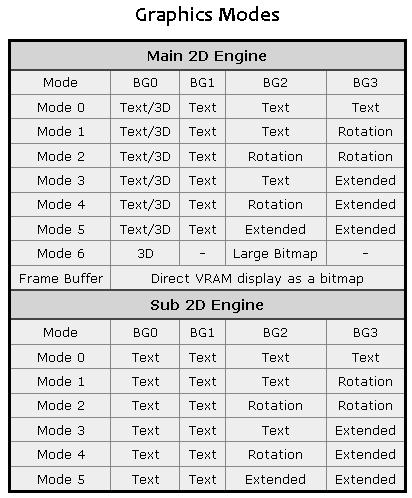
\includegraphics[height=9cm]{Figuras/C5/c5_modos-graficos.png}
	\caption{Modulos gráficos}
	\label{fig_c5_modulos}
\end{figure}

Existen tres tipos diferentes de configuraciones para los fondos 2D, que son \textit{Text}, \textit{Rotation} y \textit{Extended Rotation} y el modo \textit{framebuffer} que pinta la imagen directamente sin utilizar fondos. A los modos \textit{Text} también se les llama modos teselados, y a los modos \textit{Rotation} también se les conoce como modos \textit{Rotoscale}.

Las imágenes que se desean mostrar en la pantalla deben ser traducidas a contenido binario, que se guardará junto con el programa y que debe ser copiado en el \textit{banco de memoria VRAM (Video RAM)} en el que está mapeada la pantalla. Mapear la pantalla a un banco de memoria significa que a la pantalla se le asigna ese banco de memoria, de forma que lo que se haya escrito en ese banco de memoria será lo que se vea en la pantalla. 

La Nintendo DS tiene 9 bancos de memoria de vídeo, que se pueden usar con diferentes propósitos. Cada de uno de estos bancos de memoria está etiquetado desde \textit{VRAM\_A} hasta \textit{VRAM\_I}. La Tabla \ref{tab_c5_NivelesDeEjecución} muestra cada uno de los bancos de memoria VRAM con su tamaño y su dirección de memoria. La cantidad total de memoria de vídeo es de 656KB. 

\begin{table}[t]
\centering
\caption{Tamaño y dirección de memoria de cada banco de memoria.}
\begin{tabular}{|l |c | c|}
\hline
Banco & Tamaño &  Dirección memoria  \\
\hline
\hline
VRAM\_A & 128KB & 0x6800000 \\
\hline
VRAM\_B & 128KB  &	0x6820000 \\
\hline
VRAM\_C & 128KB  &	0x6840000 \\
\hline
VRAM\_D	& 128KB  &	0x6860000 \\
\hline
VRAM\_E	& 64KB  &	0x6880000\\
\hline
VRAM\_F	& 16KB  &	0x6890000 \\
\hline
VRAM\_G	& 16KB  &	0x6894000\\
\hline
VRAM\_H	& 32KB & 	0x6898000 \\
\hline
VRAM\_I	& 16KB  &	0x68a0000\\
\hline
\end{tabular}
\label{tab_c5_NivelesDeEjecución}
\end{table}

% -------------------------------------------------------------
% -------------------------------------------------------------
\section{El registro \textit{REG\_POWERCNT}} 
El registro \textit{REG\_POWERCNT} es el encargado del encendido de todo el hardware gráfico. La Figura \ref{c5_bits_reg_powercnt} muestra el significado de algunos de sus bits. El contenido de este registro permite activar ambas pantallas y los dos motores gráficos: el principal (main) y el secundario (sub) para trabajar en 2D. Además, el bit 15  permite intercambiar ambas pantallas y asignar  el motor principal a la pantalla superior (top) en vez de a la inferior que es la que tiene por defecto.

\begin{figure}[h]
\centering
\includegraphics[height=6cm]{Figuras/C5/c5_reg_powercnt.png}
\caption{Significado de los bits del registro \textit{REG\_POWERCNT}}
\label{c5_bits_reg_powercnt}
\end{figure}

Por ejemplo, para activar ambas pantallas y únicamente el motor principal se puede usar la instrucción:
\begin{verbatim}
REG_POWERCNT = POWER_LCD | POWER_2D_A;
\end{verbatim}

Para activar ambas pantallas y ambos motores se puede usar la instrucción:
\begin{verbatim}
REG_POWERCNT = POWER_LCD | POWER_2D_A | POWER_2D_B;
\end{verbatim}

% -------------------------------------------------------------
% -------------------------------------------------------------
\section{El registro \textit{REG\_DISPCNT}} 
El registro \textit{REG\_DISPCNT} es el que se encarga de controlar los modos y fondos activos. La Figura \ref{fig_c5_reg_dispcnt3} muestra el significado de algunos de sus bits. Cabe destacar la finalidad de los siguientes bits:

\begin{itemize}
	\item Bits 0-2: especifican el modo gráfico. Del 0 al 6 en binario con tres bits.
	\item Bits 8-12: especifican el fondo.
	\item Bits 17-19: especifican la configuración del modo gráfico \textit{framebuffer}.
\end{itemize}

\begin{figure}[t]
\centering
\includegraphics[height=4cm]{Figuras/C5/c5_reg_dispcnt3.png}
\caption{Significado de los bits del registro \textit{REG\_DISPCNT}}
\label{fig_c5_reg_dispcnt3}
\end{figure}

Por ejemplo, para indicar que se activa el \textit{Modo 0} con el fondo \textit{BG0} se debe usar la siguiente instrucción:

\begin{verbatim}
REG_DISPCNT = MODE_0_2D | DISPLAY_BG0_ACTIVE;
\end{verbatim}

Esta operación también se puede llevar a cabo mediante la instrucción:
\begin{verbatim}
videoSetMode(MODE_0_2D);
\end{verbatim}

% -------------------------------------------------------------
% -------------------------------------------------------------
\section{Los registros \textit{VRAM\_?\_CR}} 
Cada \textit{banco VRAM} tiene un registro \textit{VRAM\_?\_CR} (donde ? puede tomar los valores de A a I) para activarlo y seleccionar su función. La Figura \ref{fig_c5_reg_vram1} muestra el significado de cada uno de sus bits. Cabe destacar que los bits etiquetados con \textit{Modo} y \textit{Desplazamiento} son los que permiten seleccionar la función del fondo configurado en el registro \textit{REG\_DISPCNT}. Por su parte el \textit{bit 7} es el que permite activar el correspondiente \textit{banco VRAM}.

\begin{figure}[t]
\centering
\includegraphics[height=4cm]{Figuras/C5/c5_reg_vram1.png}
\caption{Significado de los bits del registro \textit{VRAM\_X\_CR}}
\label{fig_c5_reg_vram1}
\end{figure}

Como ejemplo, para indicar que se activa \textit{VRAM\_A} y que se asigna a fondos del motor principal (\textit{main}) se debe usar la instrucción:

\begin{verbatim}
VRAM_A_CR = VRAM_A_ENABLE | VRAM_A_MAIN_BG;
\end{verbatim}

Esta operación también se podría llevar a cabo mediante:

\begin{verbatim}
vramSetBankA(VRAM_A_MAIN_BG);
\end{verbatim}

 %
%\chapterimage{chapter_head_1.pdf} 
\chapter{El modo framebuffer}

Este capítulo explica el funcionamiento del modo framebuffer. La lista de ejercicios y el tiempo estimado (en minutos) para su realización se muestran en la Tabla \ref{c6_tab:ejercios}.

\begin{table}[t]
	\centering
	\caption{Ejercicios del capítulo y tiempo estimado para su realización.}
	\begin{tabular}{|c|c|}
		\hline 
		Ejercicio & Tiempo \\ 
		\hline 
		6.1 & 20' \\ 
		6.2 & 15' \\ 
		6.3 & 25' \\ 
		6.4 & 15' \\ 
		6.5 & 15' \\ 
		6.6 & 30' \\ 
		\hline 
	\end{tabular} 
	\label{c6_tab:ejercios}
\end{table}

% -----------------------------------------------------
% -----------------------------------------------------
% -----------------------------------------------------
% -----------------------------------------------------
\section{El modo Framebuffer}
La principal peculiaridad de este modo de representación es que la pantalla se mapea directamente a la memoria, sin utilizar el motor de renderizado, de forma que lo que se escribe en memoria es lo que se muestra. Además el modo Framebuffer solo está disponible para el motor principal. 

La pantalla se compone de $49\ 152$ píxeles, organizados en 192 líneas de 256 píxeles cada una, donde a su vez, el contenido de cada píxel representa un color en formato RGB de 16 bits.

El formato RGB de 16 bits para especificar el color se representa como una mezcla de una cantidad determinada del color rojo (R), verde (G) y azul (B), dedicando 5 bits para determinar esa cantidad: 0 indica ausencia de color y el 31 el máximo color. La librería \textit{libnds} proporciona la macro \textit{RBG15} para facilitar la definición de colores. Basta con indicar la cantidad de cada uno de ellos, en un rango de 0 a 31, para obtener el color en formato RGB de 16 bits. Por ejemplo, para obtener los colores: rojo, verde, azul y negro, habrá que usar las macros: \textit{RGB15(31,0,0)}, \textit{RGB15(0,31,0)}, \textit{RGB15(0,0,31)}, \textit{RGB15(0,0,0)}, respectivamente. El uso de esta macro simplifica bastante la tarea de dibujado en la pantalla, ya que únicamente hay que asignar píxel a píxel el valor correspondiente al color que
se desea pintar.

Tal como muestra la Figura \ref{fig_c5_modulos} únicamente el motor principal puede usar el modo framebuffer. Esto implica que solo se podrá mostrar una imagen en una de las dos pantallas a la vez.
% -----------------------------------------------------
% -----------------------------------------------------
\section{Preparando el modo framebuffer}
El modo framebuffer admite cuatro tipos de configuración, que reciben el nombre de FB0, FB1, FB2 o FB3 y que básicamente establecen la zona de memoria cuyo contenido se va a volcar en la pantalla. Las zonas de memoria donde se deberá volcar la información en cada una de las cuatro configuraciones son VRAM\_A, VRAM\_B, VRAM\_C o VRAM\_D, respectivamente.

En primer lugar hay que especificar el modo seleccionado, para lo cual se utiliza el registro REG\_DISPCNT y la macro que se corresponda con el modo a utilizar. Por ejemplo, para usar la configuración FB0 (y por lo tanto la zona de memoria VRAM\_A) se deberá usar el siguiente código:

\begin{verbatim}
REG_DISPCNT = MODE_FB0;
\end{verbatim}

Al especificar el modo de vídeo, indirectamente se está especificando la zona de memoria donde se deberán escribir los datos que se van a mostrar en la pantalla. Para poder utilizar los bancos de memoria es necesario que éstos estén habilitados y configurados según su finalidad. Para ello hay que usar el siguiente código:

\begin{verbatim}
VRAM_A_CR = VRAM_ENABLE | VRAM_A_LCD;
\end{verbatim}

Una vez especificado el modo y habilitada la zona de memoria donde se escribirán los datos, el siguiente paso consiste en escribir en la memoria el valor que se asignará a cada uno de los píxeles de la pantalla, bien mediante una asignación manual, utilizando la macro RGB15 o escribiendo los datos correspondientes a una imagen específica.

% -----------------------------------------------------
% -----------------------------------------------------
\section{Mostrar imágenes}
\label{sec:p2_c3_imagenes}
El modo framebuffer no utiliza fondos ni motor de renderizado, por lo que la única tarea a realizar para mostrar una imagen es transferir al banco de memoria correspondiente los datos del gráfico a mostrar. Para ello, será necesario convertir esa imagen en un mapa de bits.

La conversión de imágenes se realiza con la herramienta \textit{grit}, que ya viene integrada en \textit{devkitPro}. En concreto, el comando \textit{grit} se encuentra en el directorio \textit{devkitPro/tools/bin/grit.exe} \footnote{En versiones anteriores se encontraba en \textit{devkitPro/devkitARM/bin/grit.exe}}. Por ejemplo, para convertir la imagen \textit{imagen.png} al formato que se necesita, se deberá ejecutar la siguiente orden:

\begin{verbatim}
grit imagen.png -gb -gB16
\end{verbatim}

La primera opción (-gb) indica que el formato de la conversión es un mapa de bits y la segunda opción (-gB16), que tiene una profundidad de 16 bits por píxel.

El comando creará un fichero de cabecera \textit{imagen.h} y un fichero \textit{imagen.s} que contiene el vector de datos correspondiente al mapa de bits de la imagen especificada (en lenguaje ensamblador ARM). El fichero de cabecera deberá ser incluido en el programa principal con la orden:

\begin{verbatim}
#include "imagen.h"
\end{verbatim}
	
El fichero \textit{imagen.s} deberá ser añadido al proyecto para que el linker puede añadir la imagen al ejecutable.

\begin{example}
El siguiente programa (\textit{unaimagen.c}) muestra la imagen \textit{mario.png} en la pantalla inferior de la NDS:

\begin{lstlisting}
#include <nds.h>
#include "mario.h"

int main (void)
{
	REG_POWERCNT = POWER_LCD | POWER_2D_A;
	REG_DISPCNT  = MODE_FB0;
	VRAM_A_CR    = VRAM_ENABLE | VRAM_A_LCD;
	dmaCopy(marioBitmap, VRAM_A, 256*192*2);
	while (1)
	{
		swiWaitForVBlank();
	}
	return 0;
}
\end{lstlisting}
\end{example}

La función \textit{dmaCopy} se encarga de copiar el vector de datos \textit{marioBitmap} (declarado en mario.h) al banco de memoria (VRAM\_A) que está mapeado a la pantalla.

\begin{exercise}
Crea un nuevo proyecto, usando como punto de partida el programa \textit{unaimagen.c}, que muestre en la pantalla inferior una imagen de 256*192 píxeles. Recuerda que debes obtener los ficheros \textit{.h} y \textit{.c} de la imagen usando el comando \textit{grit} y que dichos ficheros deben estar incluidos en el proyecto.
\end{exercise}


\begin{example}
En el siguiente programa (\textit{dosimagenes.c}) se cargan dos imágenes (una en VRAM\_A y la otra en VRAM\_B). Cuando se pulsa la tecla A (de la NDS) se mostrará una de ellas, cuando se pulsa la tecla X (de la NDS) se mostrará la otra:

\begin{lstlisting}
#include <nds.h>
#include "mario.h"
#include "wallpaper.h"

int main (void)
{
	REG_POWERCNT = POWER_LCD | POWER_2D_A;
	
	VRAM_A_CR    = VRAM_ENABLE | VRAM_A_LCD;
	dmaCopy(marioBitmap, VRAM_A, 256*192*2);
	
	VRAM_B_CR    = VRAM_ENABLE | VRAM_B_LCD;
	dmaCopy(wallpaperBitmap, VRAM_B, 256*192*2);
	
	// De inicio se muestra la que se encuentra en VRAM_A (FB0)
	REG_DISPCNT  = MODE_FB0;
	while (1)
	{
		scanKeys();
		int held=keysUp();
		
		if (held & KEY_A)
		{
			REG_DISPCNT  = MODE_FB0;
		}
		if (held & KEY_X)
		{
			REG_DISPCNT  = MODE_FB1;
		}
		
		swiWaitForVBlank();
	}
	return 0;
}
\end{lstlisting}
\end{example}

Como se puede comprobar, en primer lugar se carga la primera imagen en VRAM\_A y la segunda en VRAM\_B. Para seleccionar que imagen se quiere mostrar, es necesario especificarlo cambiando el contenido del registro REG\_DISPCNT. Los ficheros \textit{.s} de ambas imágenes deben estar incluidos en el proyecto.

\begin{exercise}
Crea un nuevo proyecto, usando como punto de partida el programa \textit{dosimagenes.c}, que muestre en la pantalla inferior una imagen de 256*192 píxeles. Cuando se pulse la tecla X se cambiará la imagen por otra. Si se pulsa de nuevo la tecla X, se volverá a cambiar la imagen mostrada y así sucesivamente. En total existirán 4 imágenes diferentes.
\end{exercise}

\begin{exercise}
Modifica el programa anterior para que el cambio de imagen a mostrar se realice cada un número determinado de segundos (por ejemplo cada 2 segundos). Al final del capítulo 3 hay un ejemplo que te puede servir de mucha ayuda.
\end{exercise}
	
% -----------------------------------------------------
% -----------------------------------------------------
\section{Dibujar píxeles}
\label{sec:p2_c3_pixeles}
Otra forma alternativa de representar gráficos en modo framebuffer consiste en componer una imagen a partir de la asignación de colores a cada uno de los píxeles que componen la pantalla. Al igual que en el caso anterior, el primer paso consistirá en especificar el modo de vídeo utilizado. 
	
El siguiente paso difiere del apartado anterior, donde se hacía una transferencia directa de un vector de datos, correspondiente a la imagen a dibujar. En este caso, se accederá directamente a la región de memoria VRAM utilizada, para escribir uno por uno el valor del color que se desee asignar a cada uno de los píxeles que componen la pantalla. La macro \textit{RGB15} permite obtener ese valor, indicando la cantidad de color rojo, verde y azul de la que se compone el color que se pintará en cada píxel.

\begin{example}
Supongamos que se desea mostar un degradado vertical de color negro a azul, que ocupe toda la pantalla. El color negro se obtiene mediante la ausencia de color de las tres tonalidades, por lo tanto, mediante \textit{RGB15(0,0,0)} obtenemos el valor correspondiente. Para hacer el degradado se deberá ir incrementando la cantidad de azul a medida que se vaya descendiendo en la pantalla. Dicho de otra forma, el nivel de color azul depende exclusivamente de la línea que estemos pintando. Por tanto basta con recorrer todos los puntos de la pantalla y pintarlos con el color correspondiente a la línea. El programa (\textit{degradado.c}) se podría implementar como sigue:
	
\begin{lstlisting}	
#include <nds.h>
#include <stdio.h>

int main (void)
{
	REG_POWERCNT = POWER_LCD | POWER_2D_A;
	REG_DISPCNT  = MODE_FB0;
	VRAM_A_CR    = VRAM_ENABLE | VRAM_A_LCD;
		
	int lin, col;
	unsigned short *fb = VRAM_A;
	for(lin=0; lin<192; lin ++)
		for(col=0; col<256; col ++)
			fb[lin*256 + col] = RGB15 (0, 0, lin*32/192);
		
	while(1)
	{
		swiWaitForVBlank();
	}
	return 0;
}	
\end{lstlisting}
\end{example}
	
En la línea 11 se define un puntero de tipo entero sin signo de 16 bits y se hace que éste apunte a la dirección 0x6800000 (valor de la macro VRAM\_A), que es el comienzo de la memoria del framebuffer FB0. El hecho de definir el puntero a la memoria como \textit{unsigned short} es porque en este modo se necesita direccionar la memoria píxel a píxel de la pantalla que, como ya se ha comentado anteriormente, ocupan cada uno 16 bits (5 bits por componente y el bit más significativo sin usar).

En la línea 14, se utiliza el puntero fb para acceder al píxel correspondiente a la línea \textit{lin} y a la columna \textit{col}. Dado que los píxeles se almacenan por líneas y cada línea tiene 256 puntos tendremos que multiplicar el número de línea por 256 para ir al comienzo de la fila y sumar el número de columna para llegar al píxel correspondiente de la pantalla. 


\begin{exercise}
Modifica el programa anterior para que el degradado sea horizontal en vez de vertical. Para hacer el degradado se deberá ir incrementando la cantidad de azul a medida que se vaya desplazando hacia la derecha en la pantalla. Es decir, el nivel de color azul depende exclusivamente de la columna que estemos pintando.
\end{exercise}

\begin{example}
El siguiente programa (\textit{colores.c}) explica como cambiar la imagen que se muestra en la pantalla. Al pulsar las teclas A, X y B (de la NDS) se mostrará la pantalla de color rojo, verde y azul, respectivamente. El código se muestra a continuación:

\begin{lstlisting}	
#include <nds.h>
#include <stdio.h>

int main (void)
{
	
	REG_POWERCNT = POWER_LCD | POWER_2D_A;
	VRAM_A_CR    = VRAM_ENABLE | VRAM_A_LCD;
	VRAM_B_CR    = VRAM_ENABLE | VRAM_B_LCD;
	VRAM_C_CR    = VRAM_ENABLE | VRAM_A_LCD;
	
	u16 color_rojo  = RGB15(31,0,0);
	u16 color_verde = RGB15(0,31,0);
	u16 color_azul  = RGB15(0,0,31);
	
	unsigned short *fbA = VRAM_A;
	unsigned short *fbB = VRAM_B;
	unsigned short *fbC = VRAM_C;
	
	int lin,col;
	
	for(lin = 0; lin < 192; lin ++)
		for(col = 0; col < 256; col ++)
			fbA[lin*256 + col] = color_rojo;
	
	for(lin = 0; lin < 192; lin ++)
		for(col = 0; col < 256; col ++)
			fbB[lin*256 + col] = color_verde;
	
	for(lin = 0; lin < 192; lin ++)
		for(col = 0; col < 256; col ++)
			fbC[lin*256 + col] = color_azul;
	
	// de inicio FB0
	REG_DISPCNT  = MODE_FB0;
	while (1)
	{
		scanKeys();
		int held=keysHeld();
		if (held & KEY_A)
		{
			REG_DISPCNT  = MODE_FB0;
		}
		if (held & KEY_X)
		{
			REG_DISPCNT  = MODE_FB1;
		}
		if (held & KEY_B)
		{
			REG_DISPCNT  = MODE_FB2;
		}
		swiWaitForVBlank();
	}
	return 0;
}
\end{lstlisting}
\end{example}


\begin{exercise}
Realiza un programa que al pulsar las teclas A, X y B (de la NDS) muestre las banderas de tres países diferentes.
\end{exercise}


% -----------------------------------------------------
% -----------------------------------------------------
\section{Ejercicios avanzados}

\begin{exercise}
Realiza un programa que permita mover un cuadrado de 25x25 píxeles por la pantalla. Para ello se usarán los botones de las flechas de la NDS. Se deberá tener en cuenta los límites de la pantalla.
\end{exercise}






 %

%----------------------------------------------------------------------------------
% REFERENCES
%----------------------------------------------------------------------------------
\chapter*{Bibliography}
\addcontentsline{toc}{chapter}{\textcolor{ocre}{Bibliography}}
\section*{Books}
\addcontentsline{toc}{section}{Books}
\printbibliography[heading=bibempty,type=book]
\section*{Articles}
\addcontentsline{toc}{section}{Articles}
\printbibliography[heading=bibempty,type=article]


\end{document}
